% Appendix A

\chapter{Network Characterizations} % Main appendix title

\label{AppendixB} % For referencing this appendix elsewhere, use \ref{AppendixA}

\lhead{Appendix B. \emph{Network Characterizations}} % This is for the header on each page - perhaps a shortened title

\section{Average Degree}

Degree $k_i$ is the number of edges connected to the node $i$. Average degree of a network $\langle k \rangle$ indicates the ratio of total number of edges, \textit{L}, to total number of nodes, \textit{N} in a graph,
\begin{equation}
\langle k \rangle = \frac{2L}{N} \;\;\;.
\end{equation} 
In order not to count each link twice, the total number of edges is divided by $\frac{N}{2}$ instead of $N$. 
 \begin{figure}[htbp]
 
  \centering
	 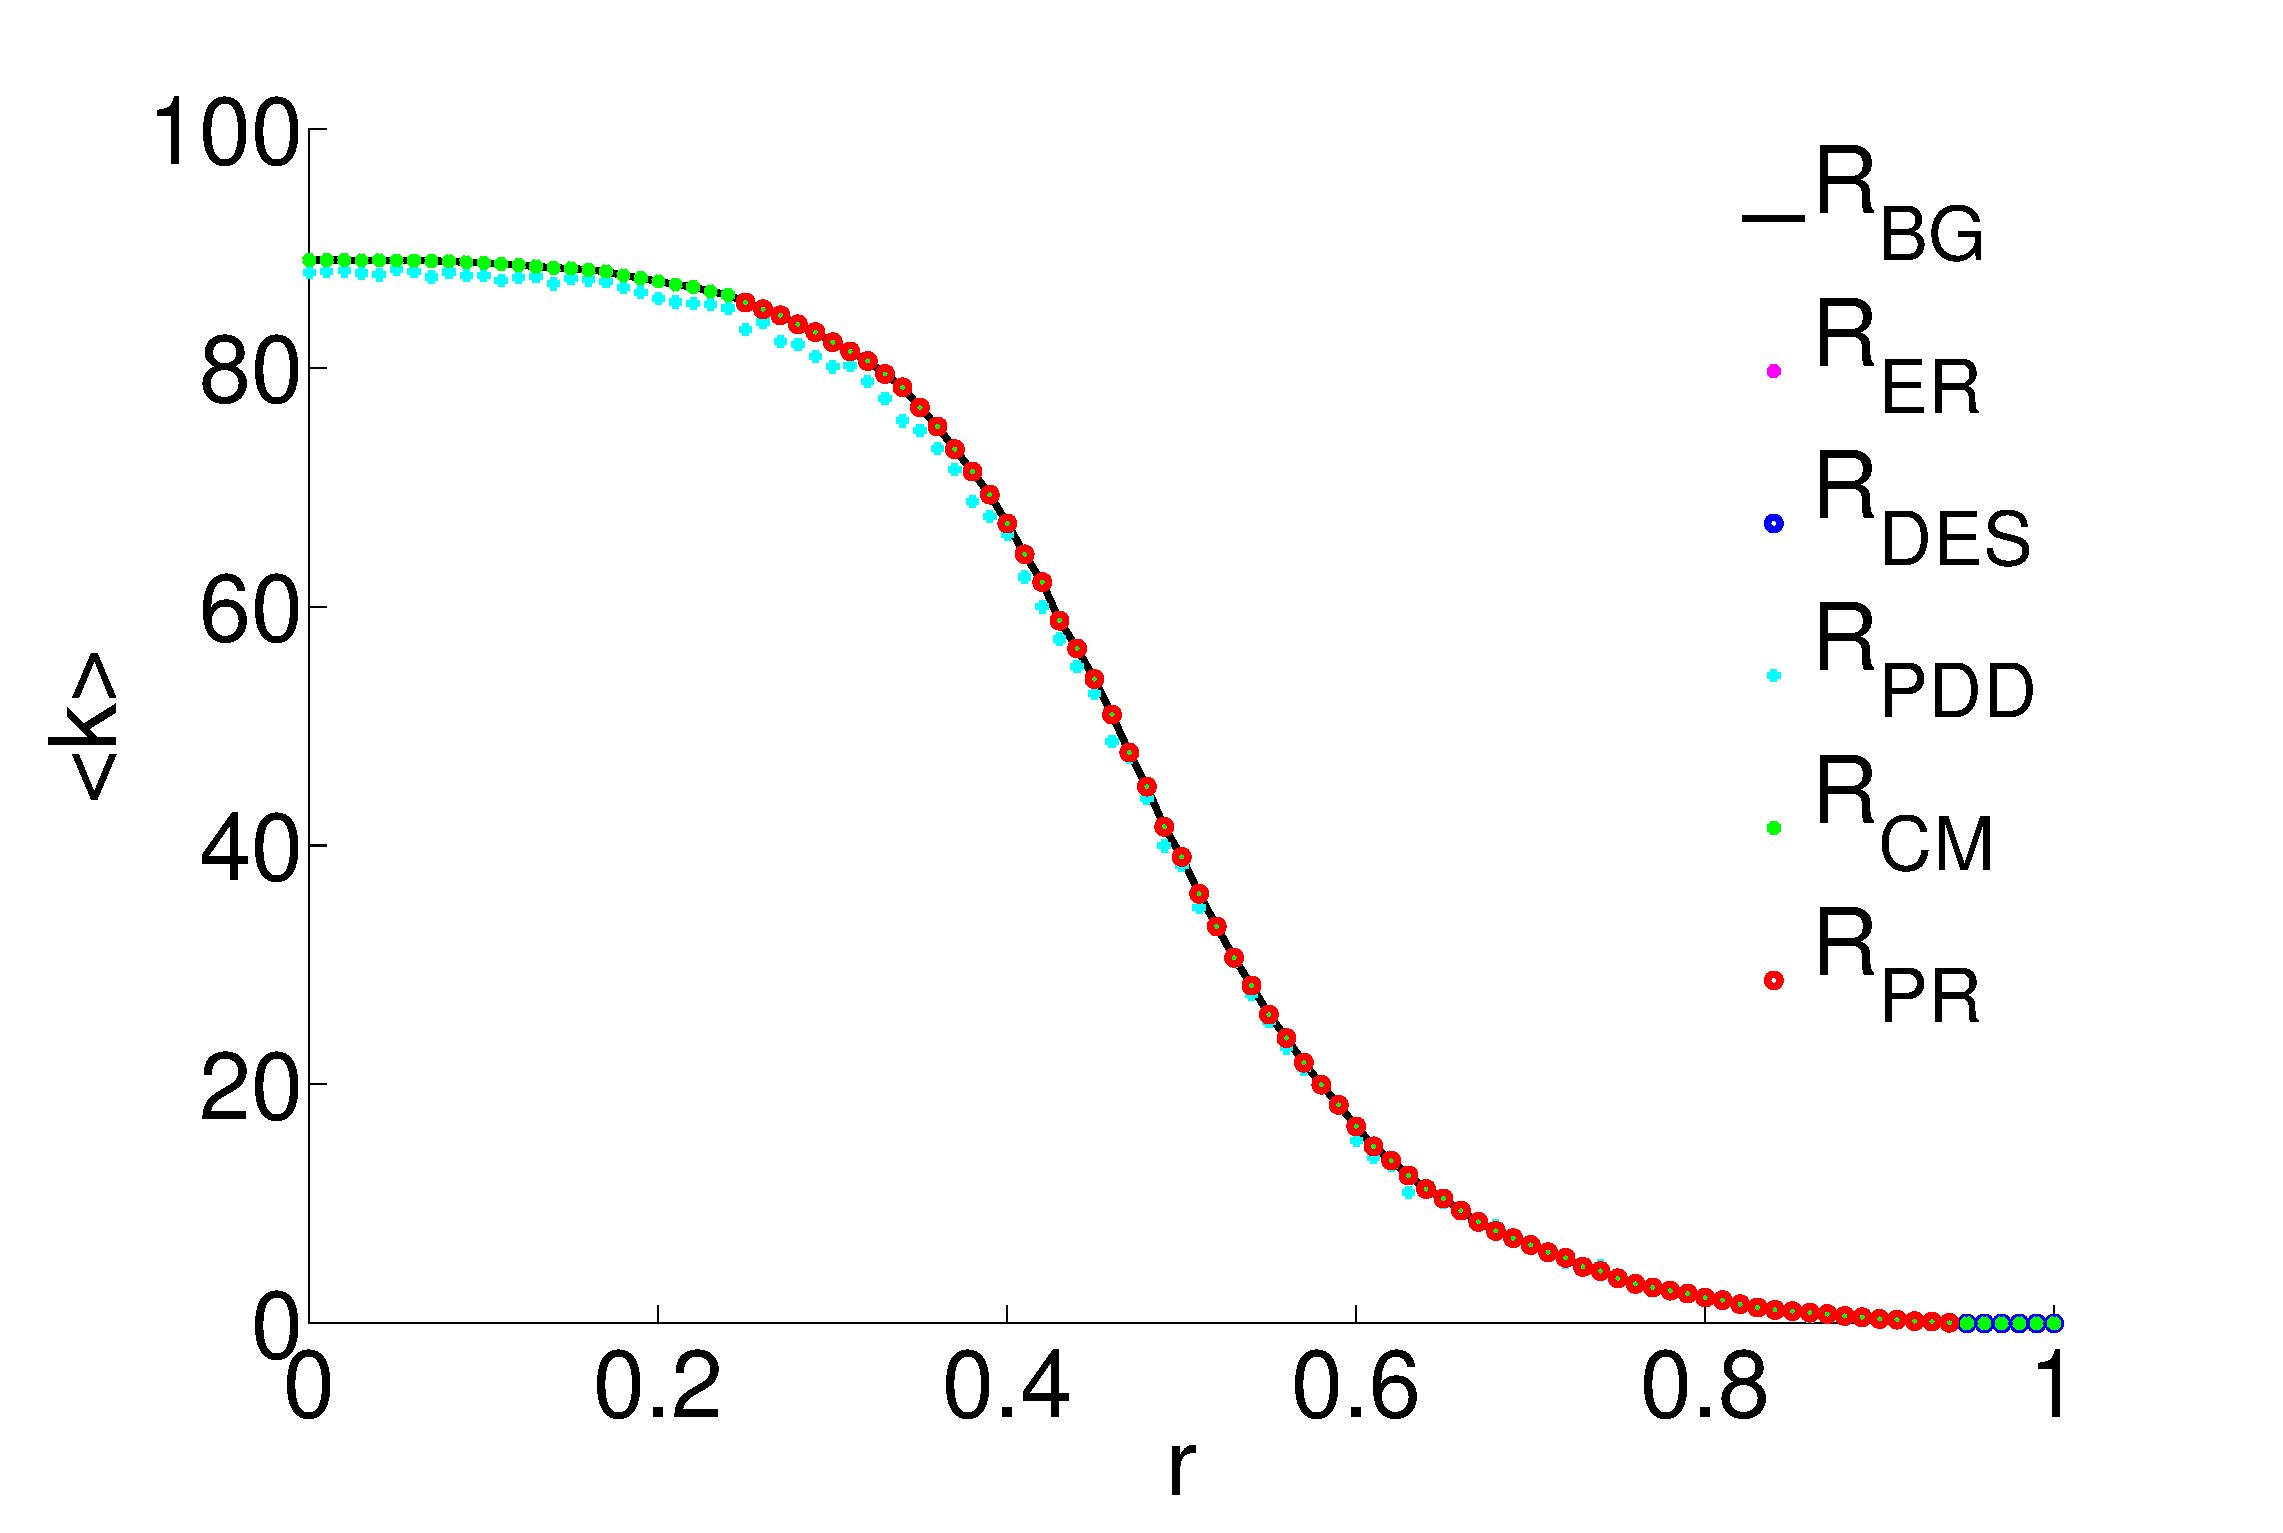
\includegraphics[width=0.49\textwidth]{Figures/Degree_Average_Fnc.eps}
	 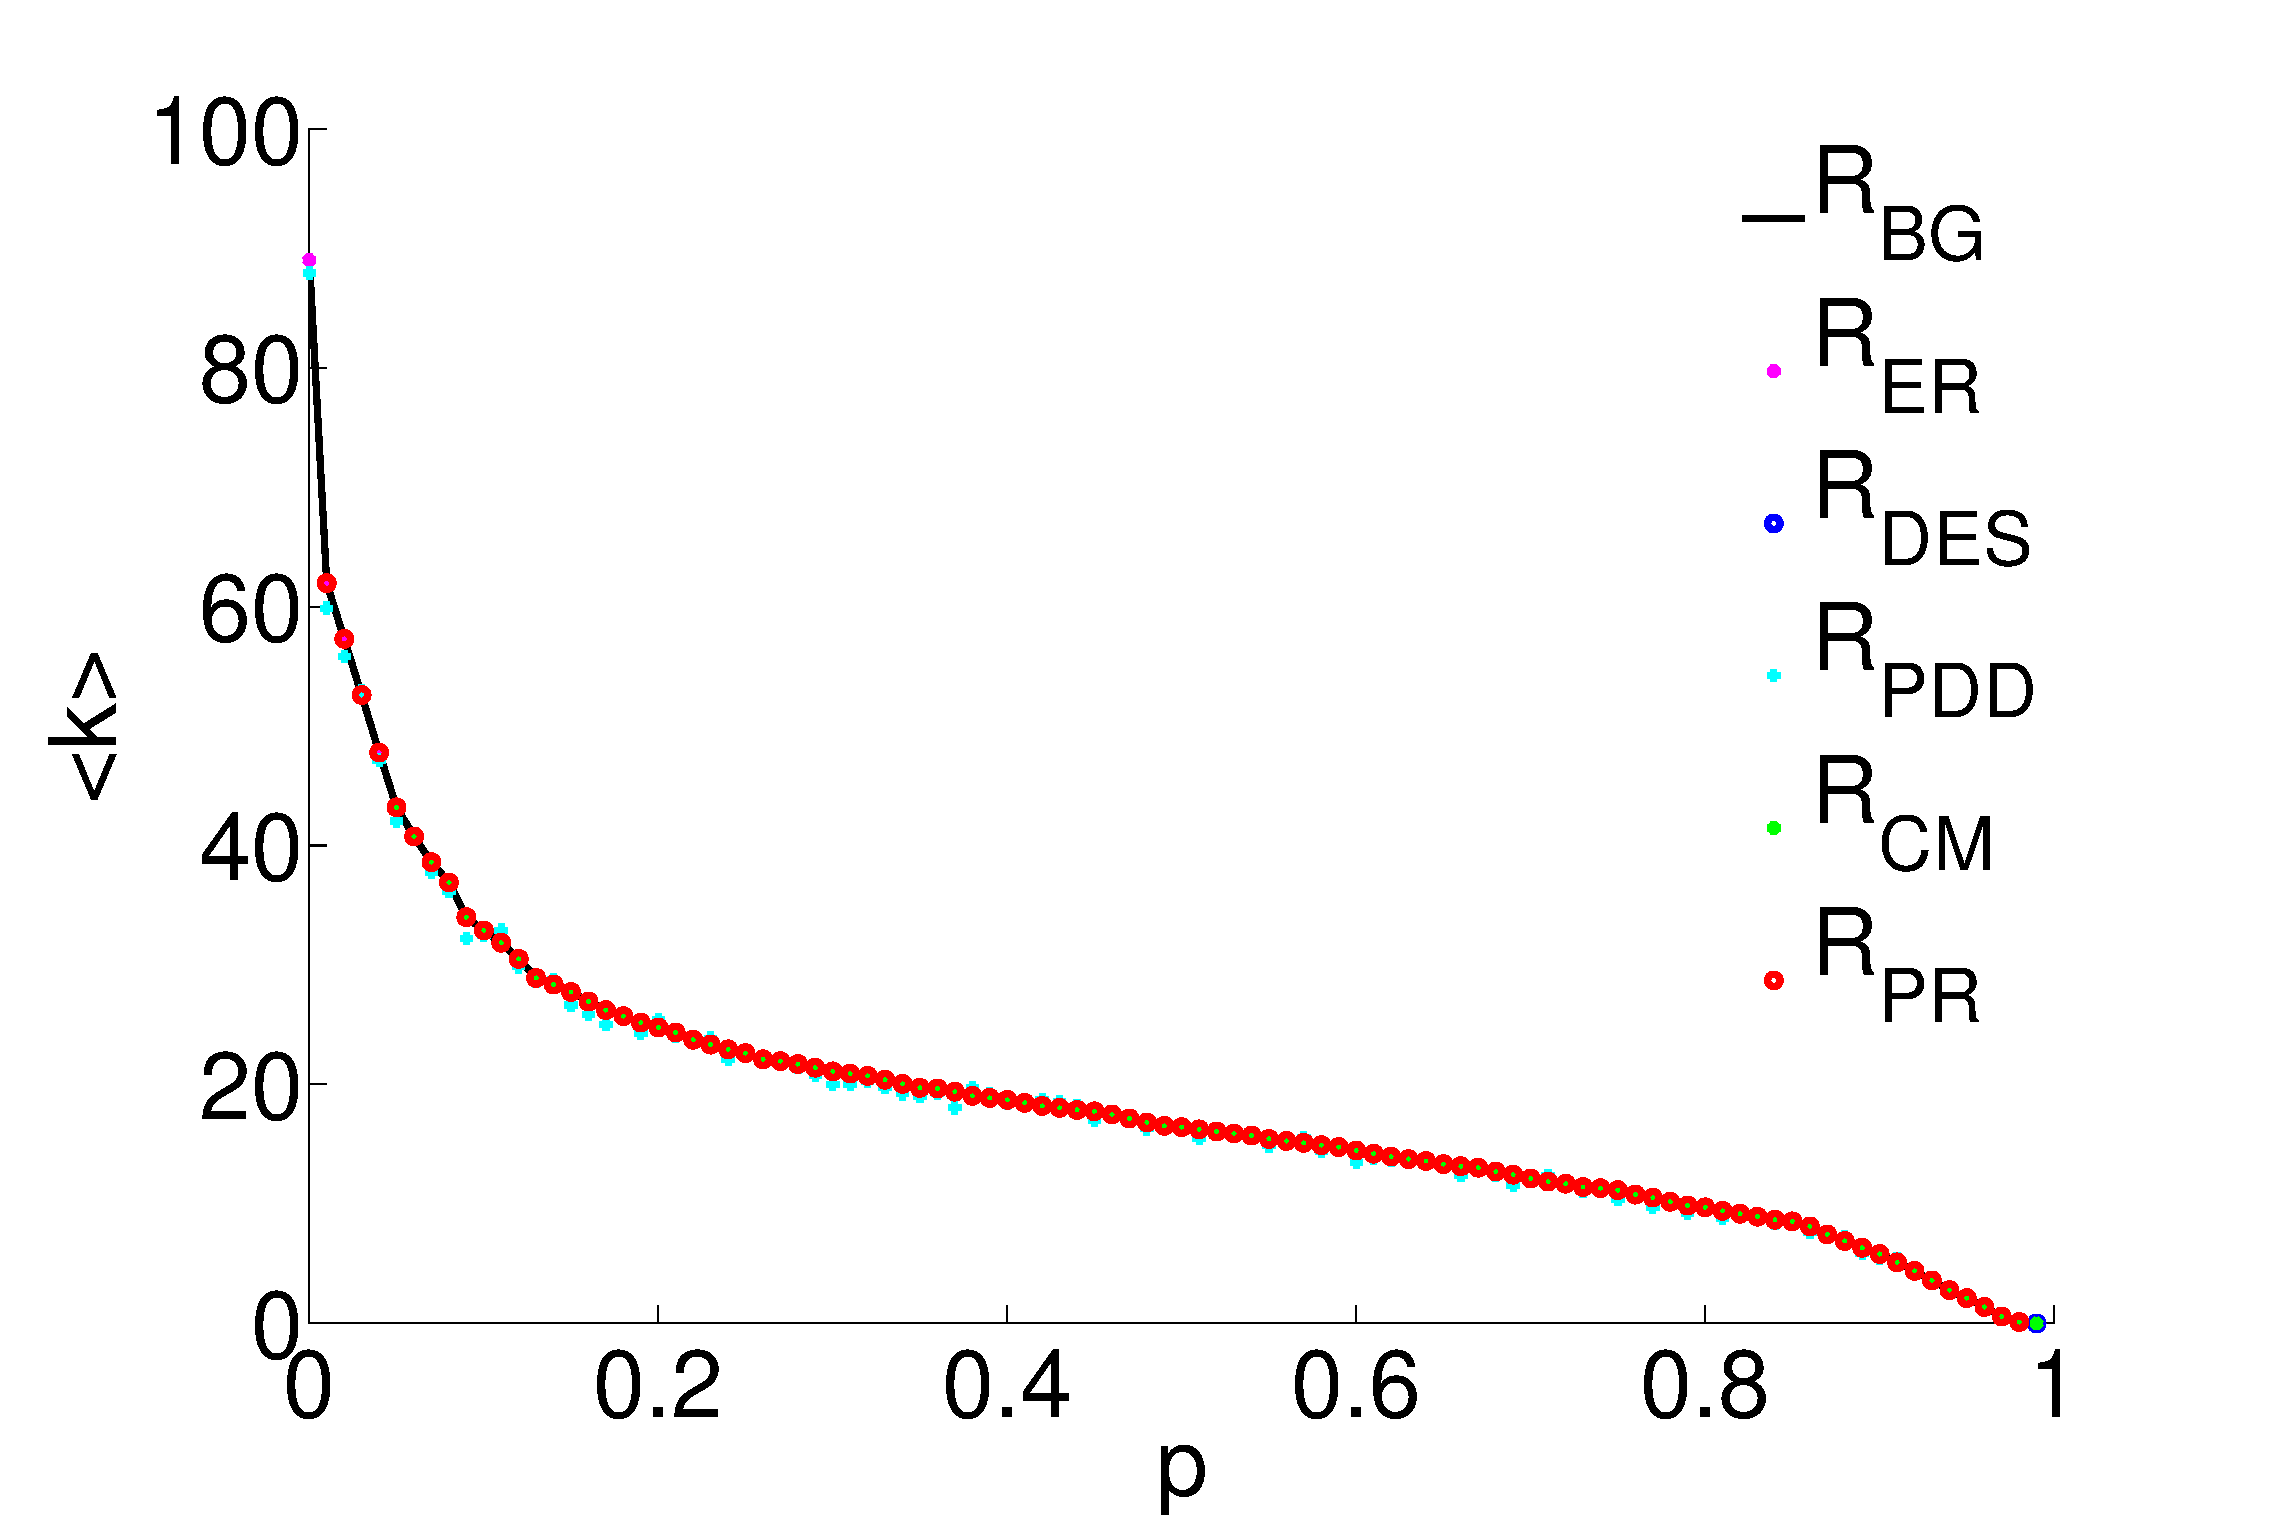
\includegraphics[width=0.49\textwidth]{Figures/Degree_Average_Stru.eps}
	\rule{35em}{0.5pt}	  
  \caption[Average Degree]{Average degrees of the brain network and the randomized networks, FC map related graphs on the left, AC map related graphs on the right. Successful $r$ ranges for randomization methods of FCM :  $r_{ER}=[0,1]$ , $r_{DES} = [0.25,1.00]$, $r_{CM} = [0,1.00]$ , $r_{PDD} = [0,1.00]$ , $r_{PR} = [0.08,0.94]$. Successful $p$ ranges of ACM : $p_{ER}=[0,0.99]$, $p_{DES}=[0.01 , 0.99]$, $p_{CM}=[0, 0.99]$ , $p_{PDD}=[0.05 , 0.98]$, $p_{PR} = [0,0.99]$.} 
    \label{fig:Average Degree}
 	
\end{figure}  


Degree is one of the statistical tools to measure the centrality of network. The higher the average degree is, the more interaction the nodes in the graph have. 

Increasing threshold and probability values diminishes number of edges inverse sigmoidally. As long as the total node numbers, total edge numbers and networks density are all preserved while constructing the random graphs, the average degree remains the same. 

\section{Average Shortest Pathway}
Shortest pathway $d_{ij}$ is a measure of integration in the network, opposite to the segregation measures. It corresponds to the shortest path length between two nodes in an unweighted graph,  
\begin{equation}
d_{ij} = \sum\limits_{a_{uv} \epsilon g_{i\leftrightarrow j} } a_{uv} \;\; ,
\end{equation}
where $g_{i\leftrightarrow j}$ is the shortest path between nodes $i$ and $j$, $d_{ij}$ is assumed to be $\infty$ for disconnected pairs \citep{RUB10}. ($d_{ij}$ is an integer here, it should not confused with distance matrix given in Appendix C.) The $d_{ij}$ 


\begin{figure}[htbp]
 
  \centering
	 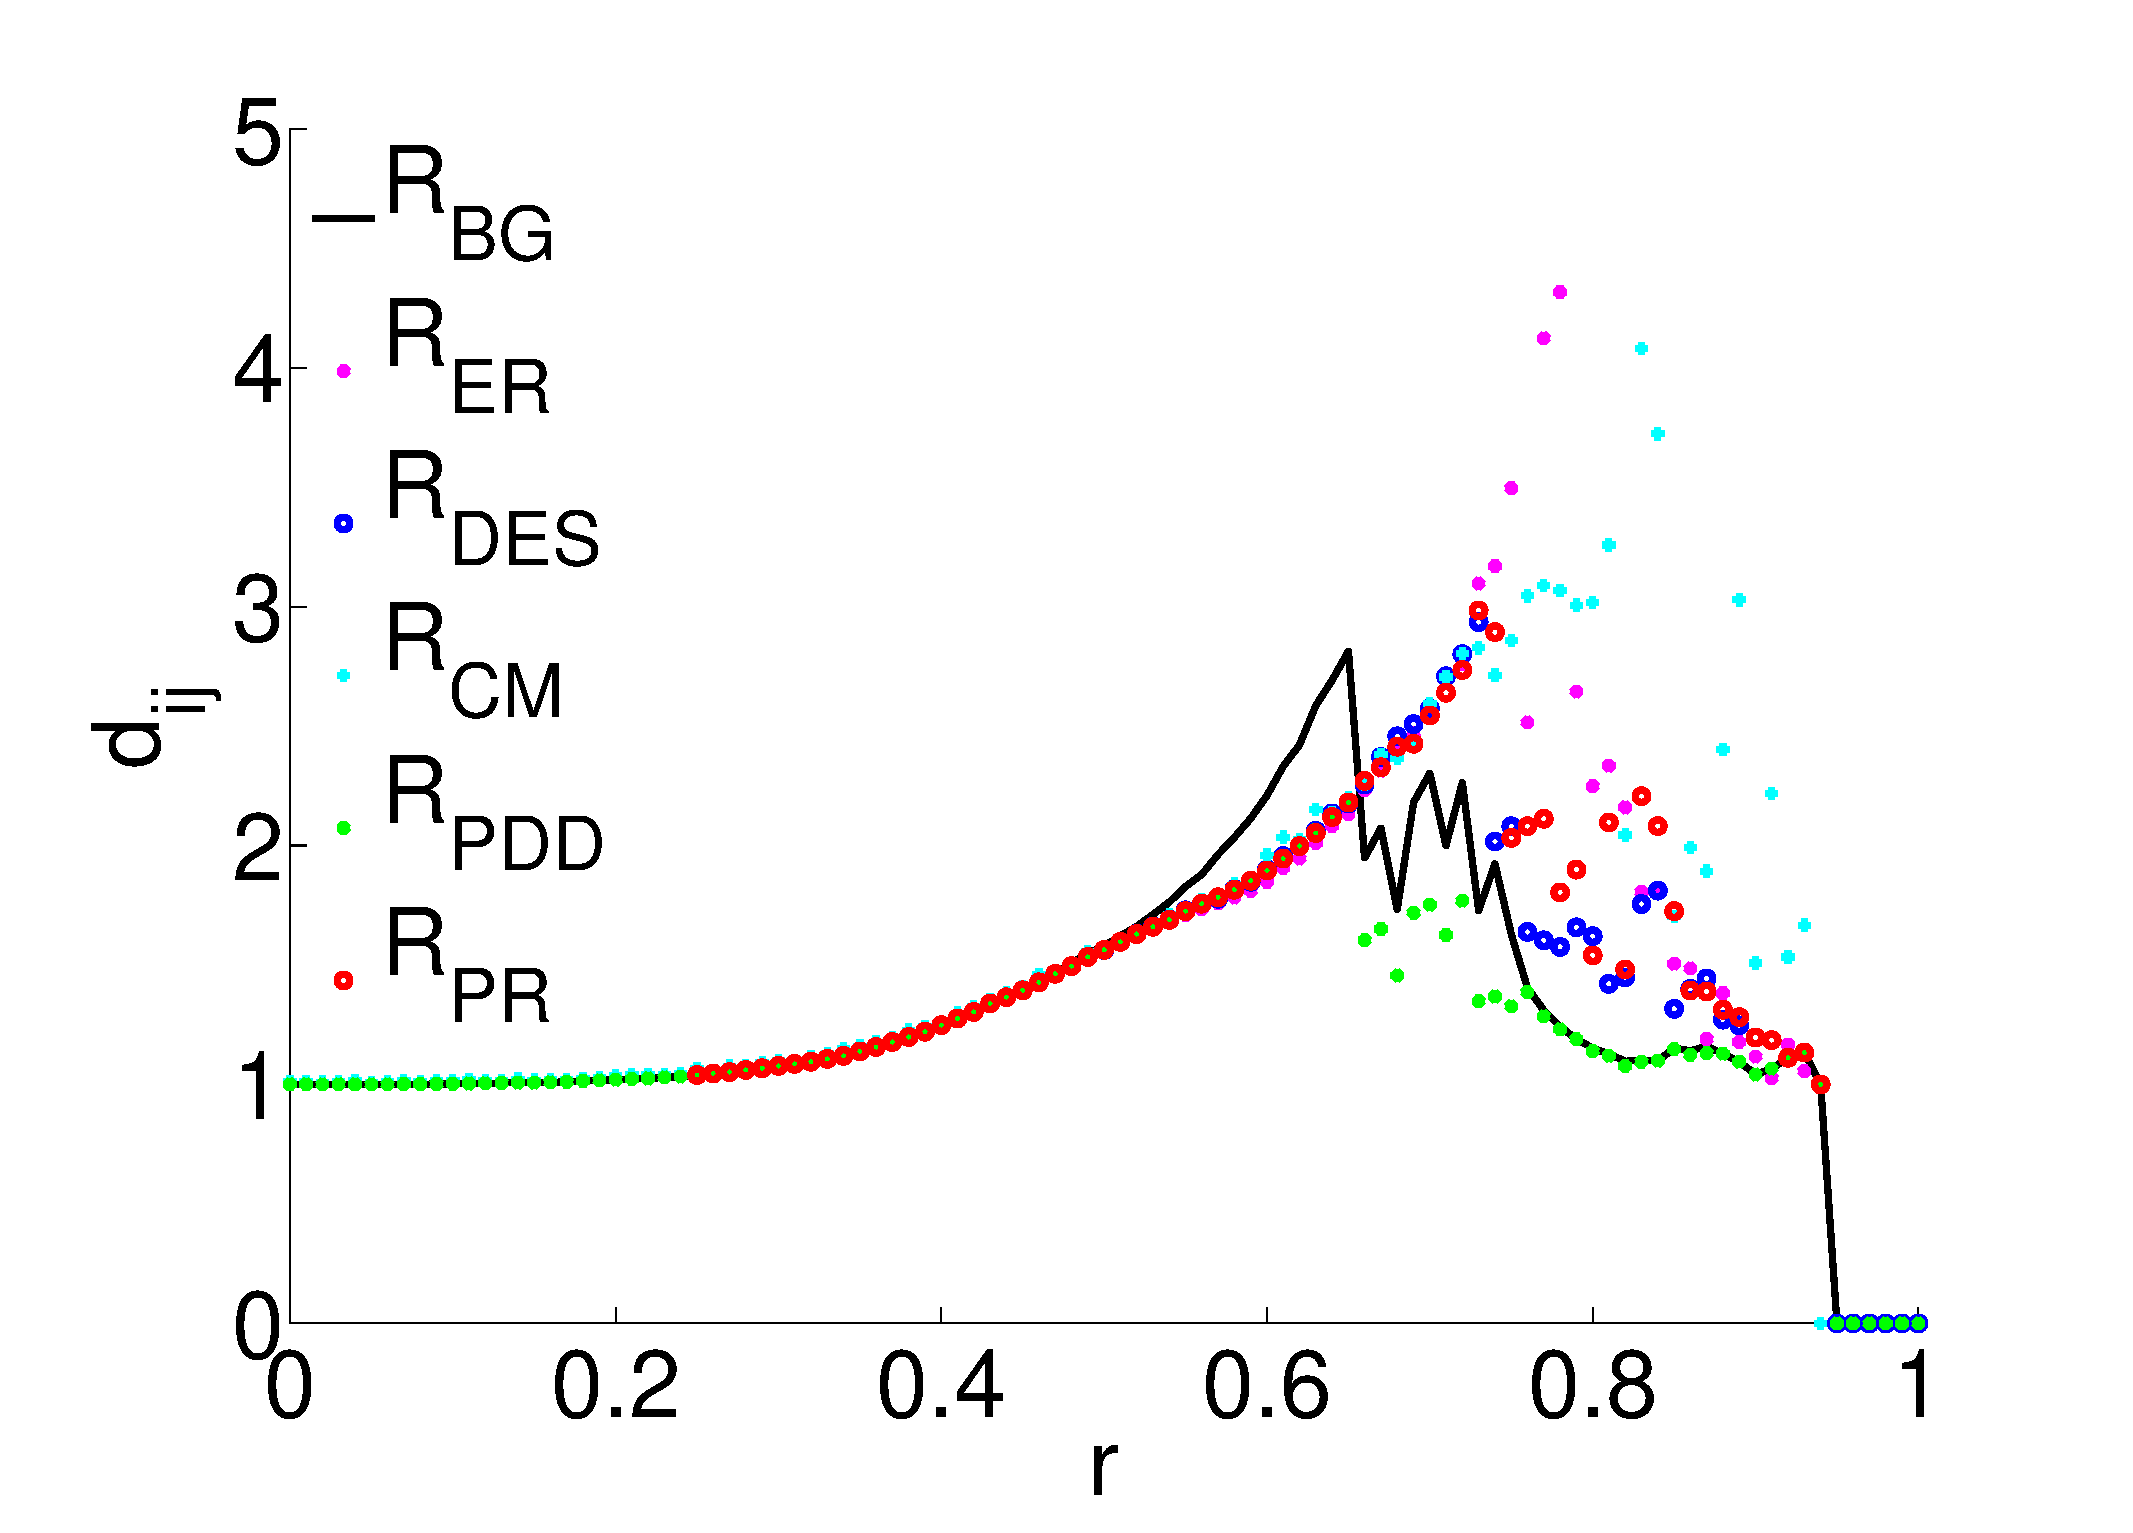
\includegraphics[width=0.49\textwidth]{Figures/Shortest_Pathway_Fnc.eps}
	 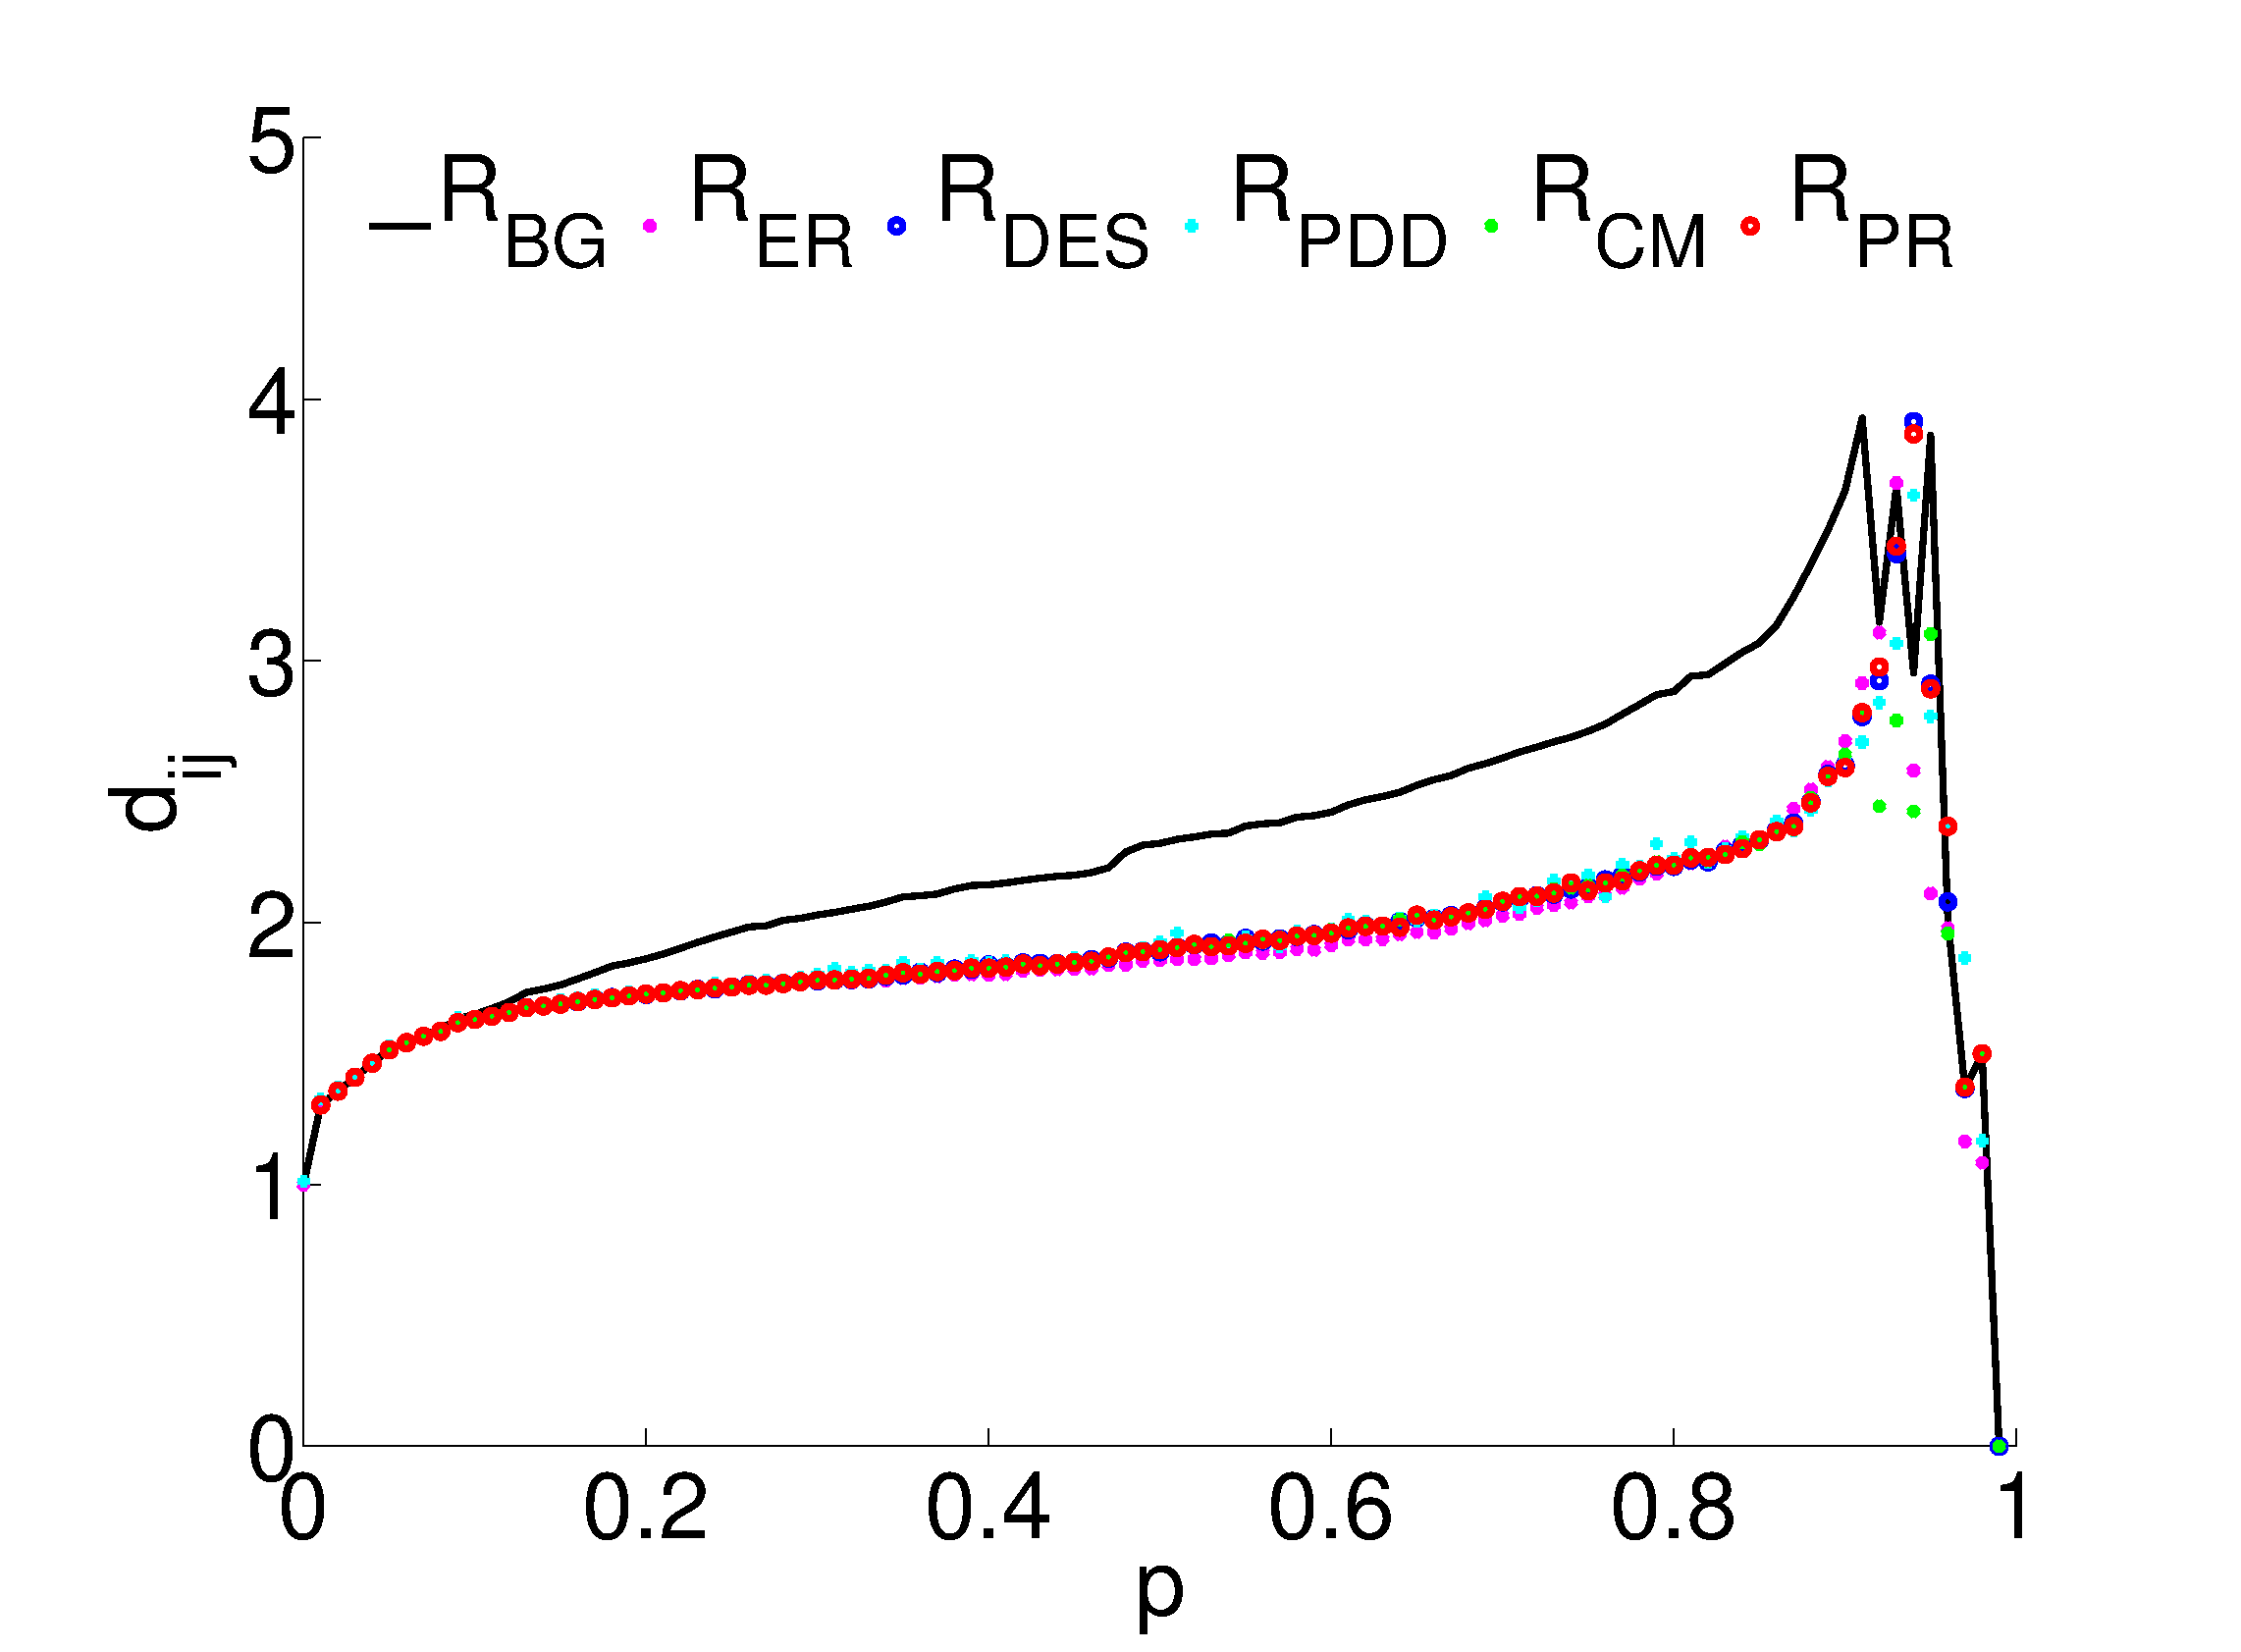
\includegraphics[width=0.49\textwidth]{Figures/Shortest_Pathway_Stru.eps}
	\rule{35em}{0.5pt}  
  \caption[Shortest Pathway]{Shortest pathway of the brain graphs and random graphs, FC map related graphs on the left and AC map related graphs on the right.} 
    \label{fig:Shortest Pathway}
 	
\end{figure}  


The $R_{BG}$ network of FCM seems to be less segregated than the randomized networks while $r$ lies between $[0.65,0.95]$. This is the threshold value at which the $R_{BG}$ network of FCM begins to get multiple components. The $R_{BG}$ network of ACM tends to be more segregated than its random networks. Whenever all the nodes get sparse (approximately $r>0.95$, $p>0.98$) in both FCM and ACM networks, the shortest pathway is represented as 0. 




\section{Global Efficiency}
The global efficiency $E$ is measured as the average of the inverse shortest pathway,

\begin{equation}
E = \frac{1}{n}\sum\limits_{i \epsilon N} E_i = \frac{1}{n}\sum\limits_{i \epsilon N} \frac{\sum\limits_{j \epsilon N, j\neq i}d_{ij}^{-1}}{n-1 } \;\, ,
\end{equation}

where $E_i$ is the global efficiency of node, $d_{ij}$ is the shortest pathway between nodes $i$ and $j$ \citep{LAT01}. As seen from the equation, global efficiency becomes larger with smaller shortest pathways between nodes. The global efficiency is a measure of the integration in the network. It reveals the strength of connections in a network. Global efficiency measures the ability of a network to transmit information at the global level \citep{XYZDA}.


\begin{figure}[htbp]
 
  \centering
	 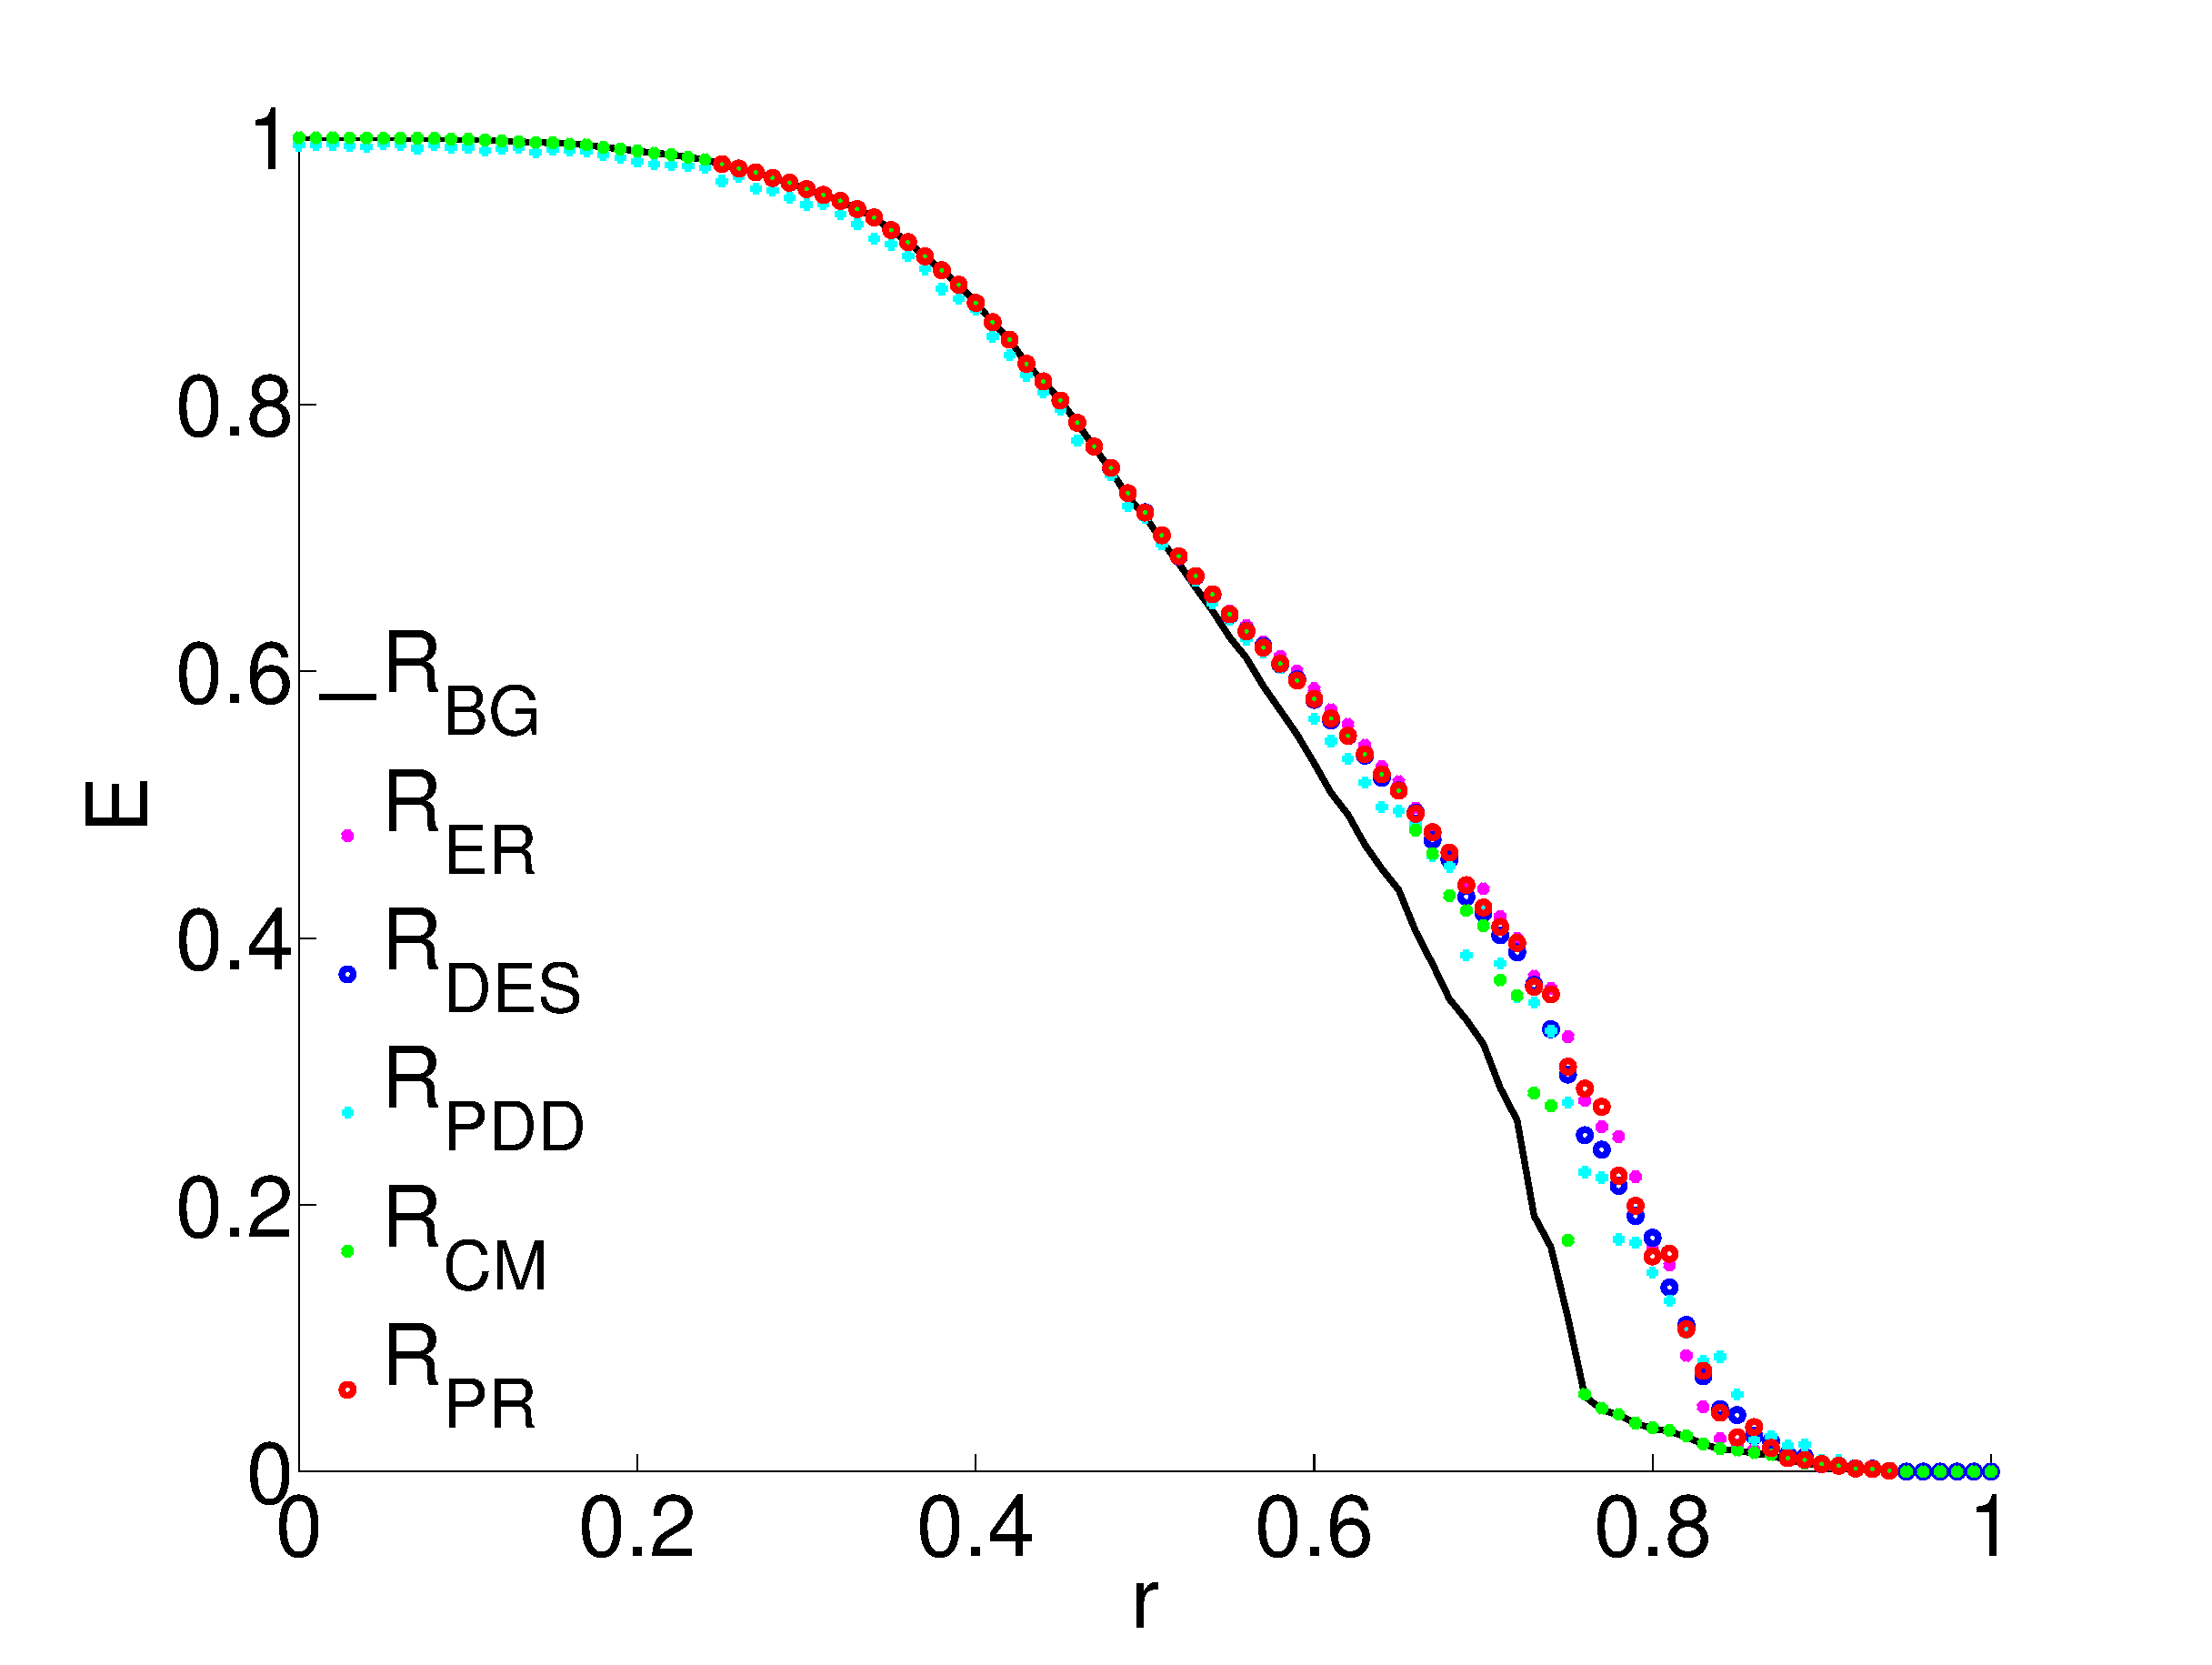
\includegraphics[width=0.49\textwidth]{Figures/Global_Efficiency_Average_Fnc.eps}
	 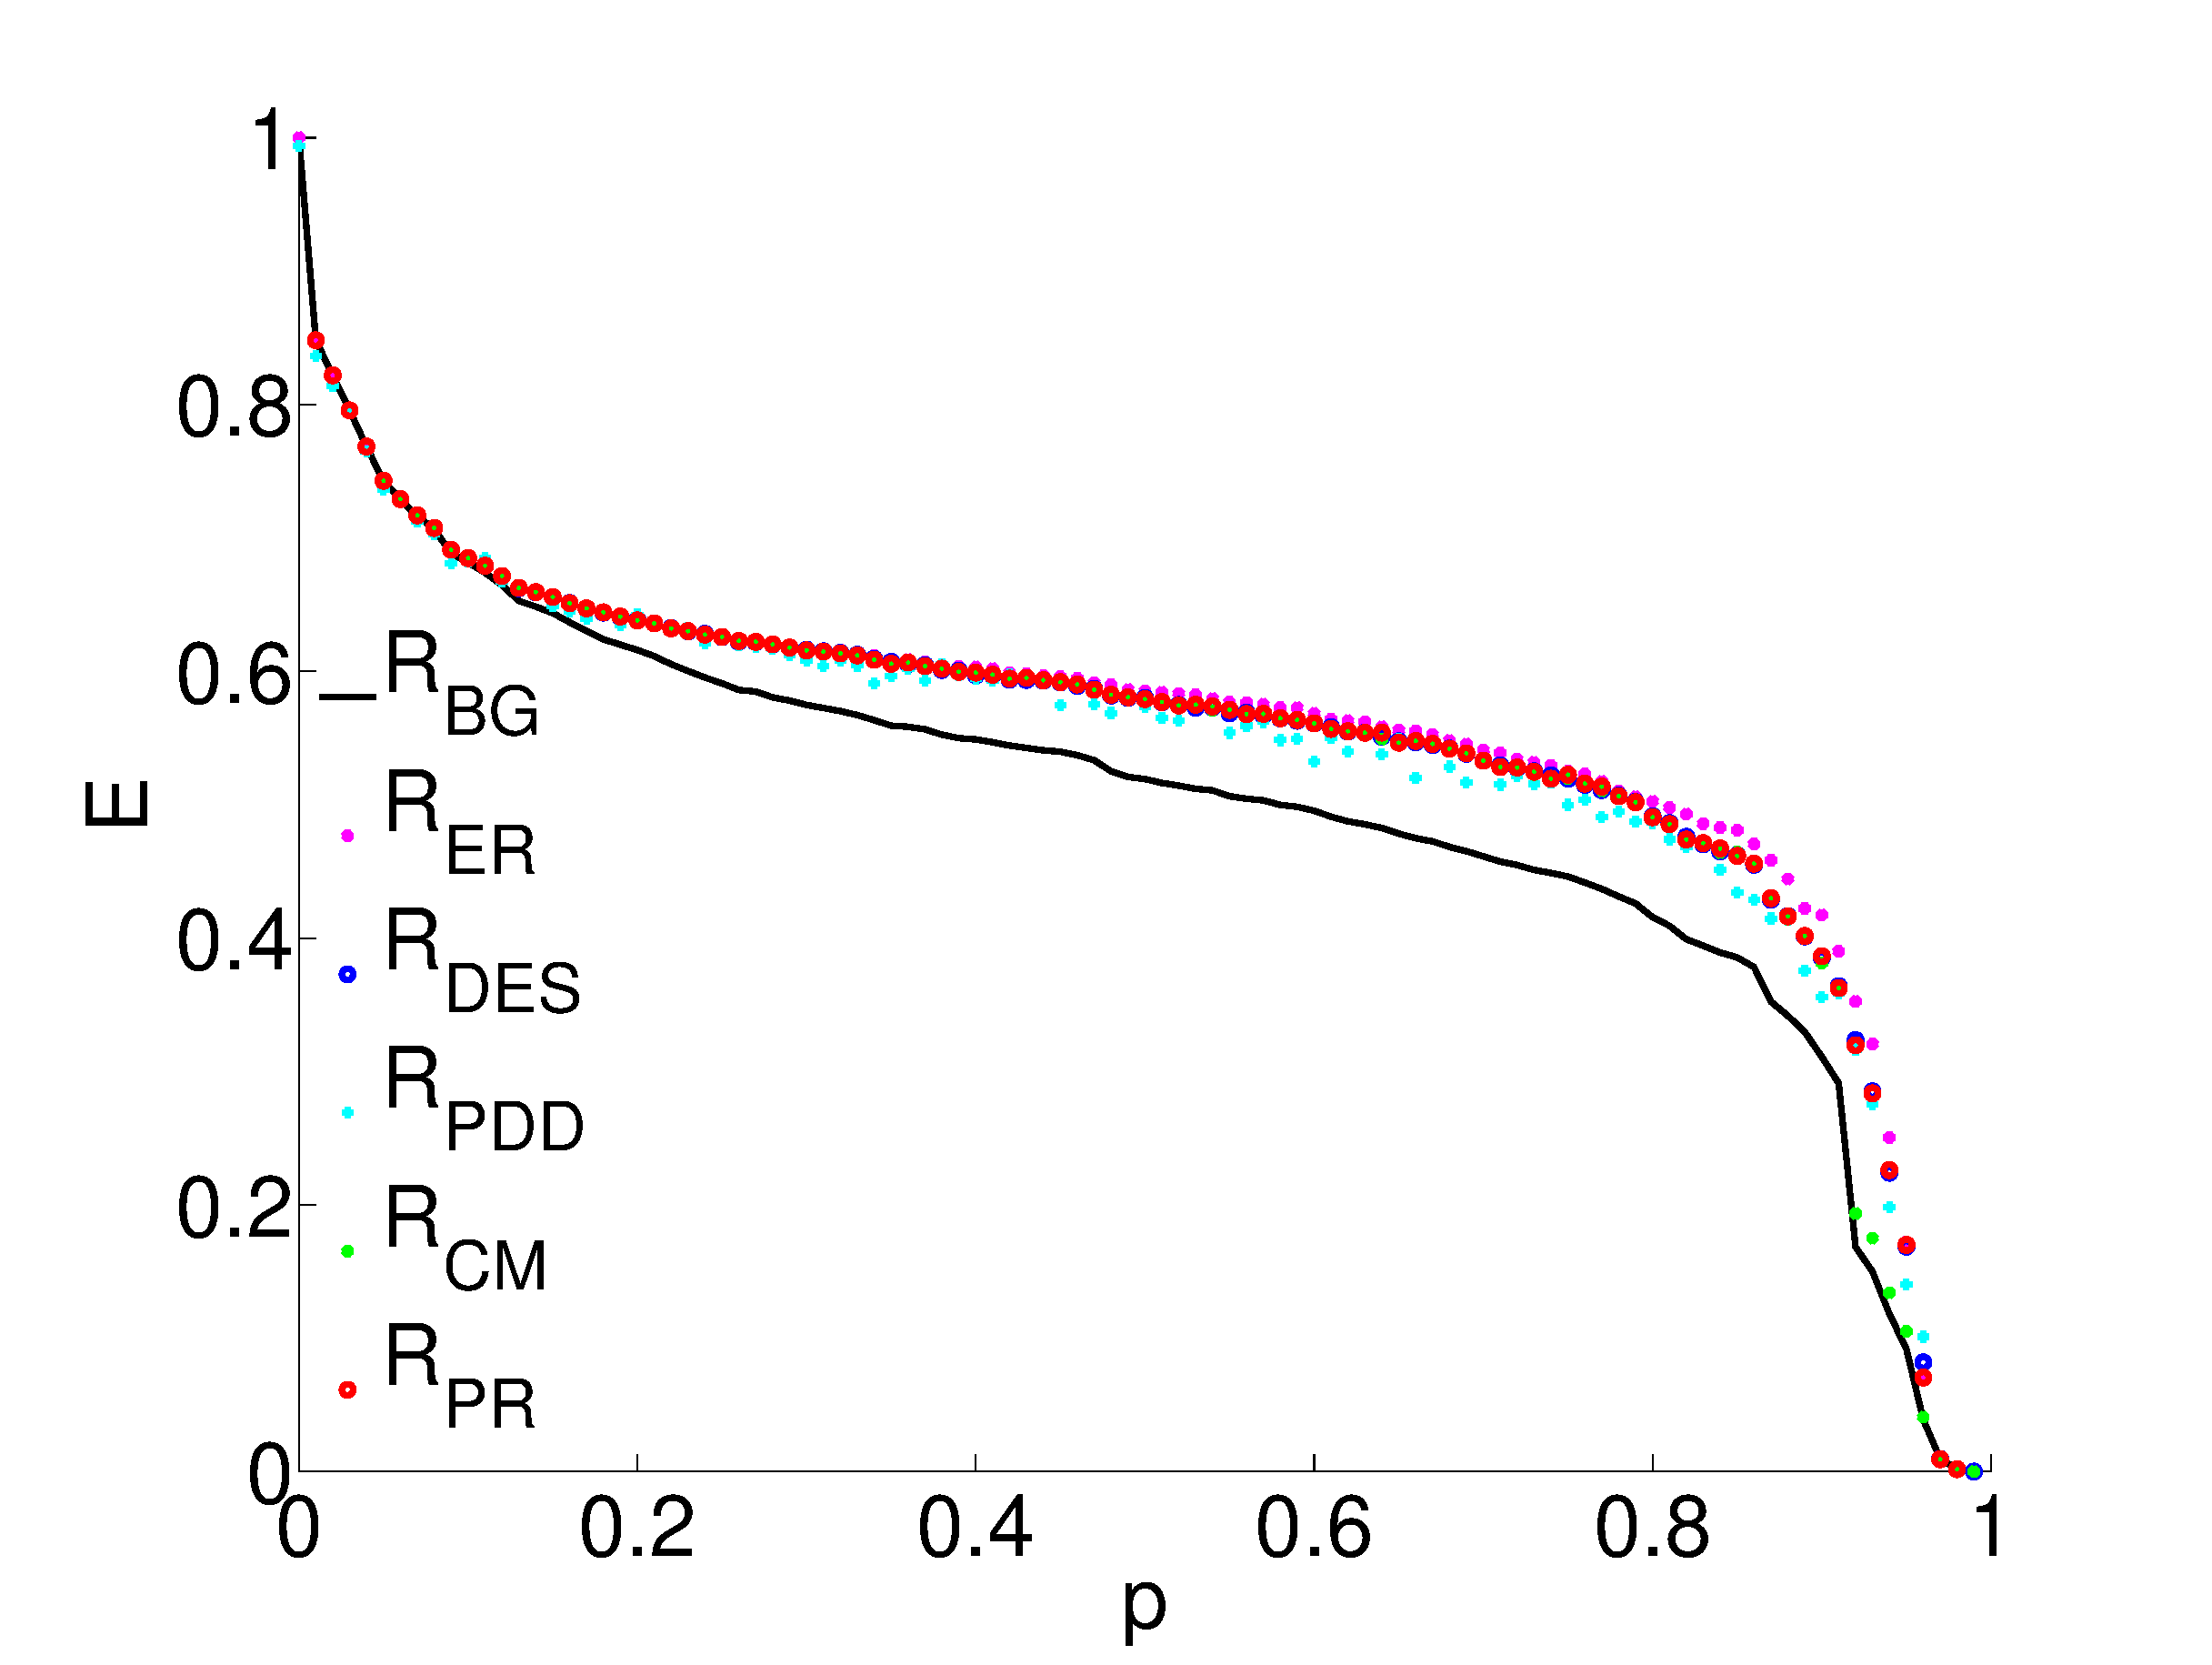
\includegraphics[width=0.49\textwidth]{Figures/Global_Efficiency_Average_Stru.eps}
	\rule{35em}{0.5pt}
  \caption[Global Efficiency]{Global efficiencies of the original networks and random graphs; FCM on left side, ACM on right side.} 
    \label{fig:Global Efficiency}
 	
\end{figure}

All randomly constructed graphs tend to have slightly higher $E$ than that of brain graphs. If it is easier to visit a node starting from any other node in the graph, the information transmission capacity is expected to be more robust. When Figure B.2 and B.3 are compared, it can be inferred that higher $d_{ij}$ values reveals lower global efficiency in a network. 



\section{Local Efficiency}
The local efficiency $E_{loc}$ is measured as the average of inverse shortest pathways between nodes in neighborhood of a specific node, 

\begin{equation}
E_{loc} = \frac{1}{n}\sum\limits_{i \epsilon N} E_{loc,i} = \frac{1}{n}\sum\limits_{i \epsilon N} \frac{\sum\limits_{j,h \epsilon N, j\neq i} a_{ij} a_{ih}[d_{jh}(N_i)]^{-1}}{k_i(k_i - 1) } \,\, ,
\end{equation}

where $E_{loc,i}$ is the local efficiency of node $i$, $d_{jh}(N_i)$ is the shortest pathway between nodes $j$ and $h$, which are located in neighborhood of node $i$ \citep{LAT01}. Local efficiency measures the ability of a network to transmit information at the local level \citep{XYZDA}.


\begin{figure}[htbp]
 
  \centering
	 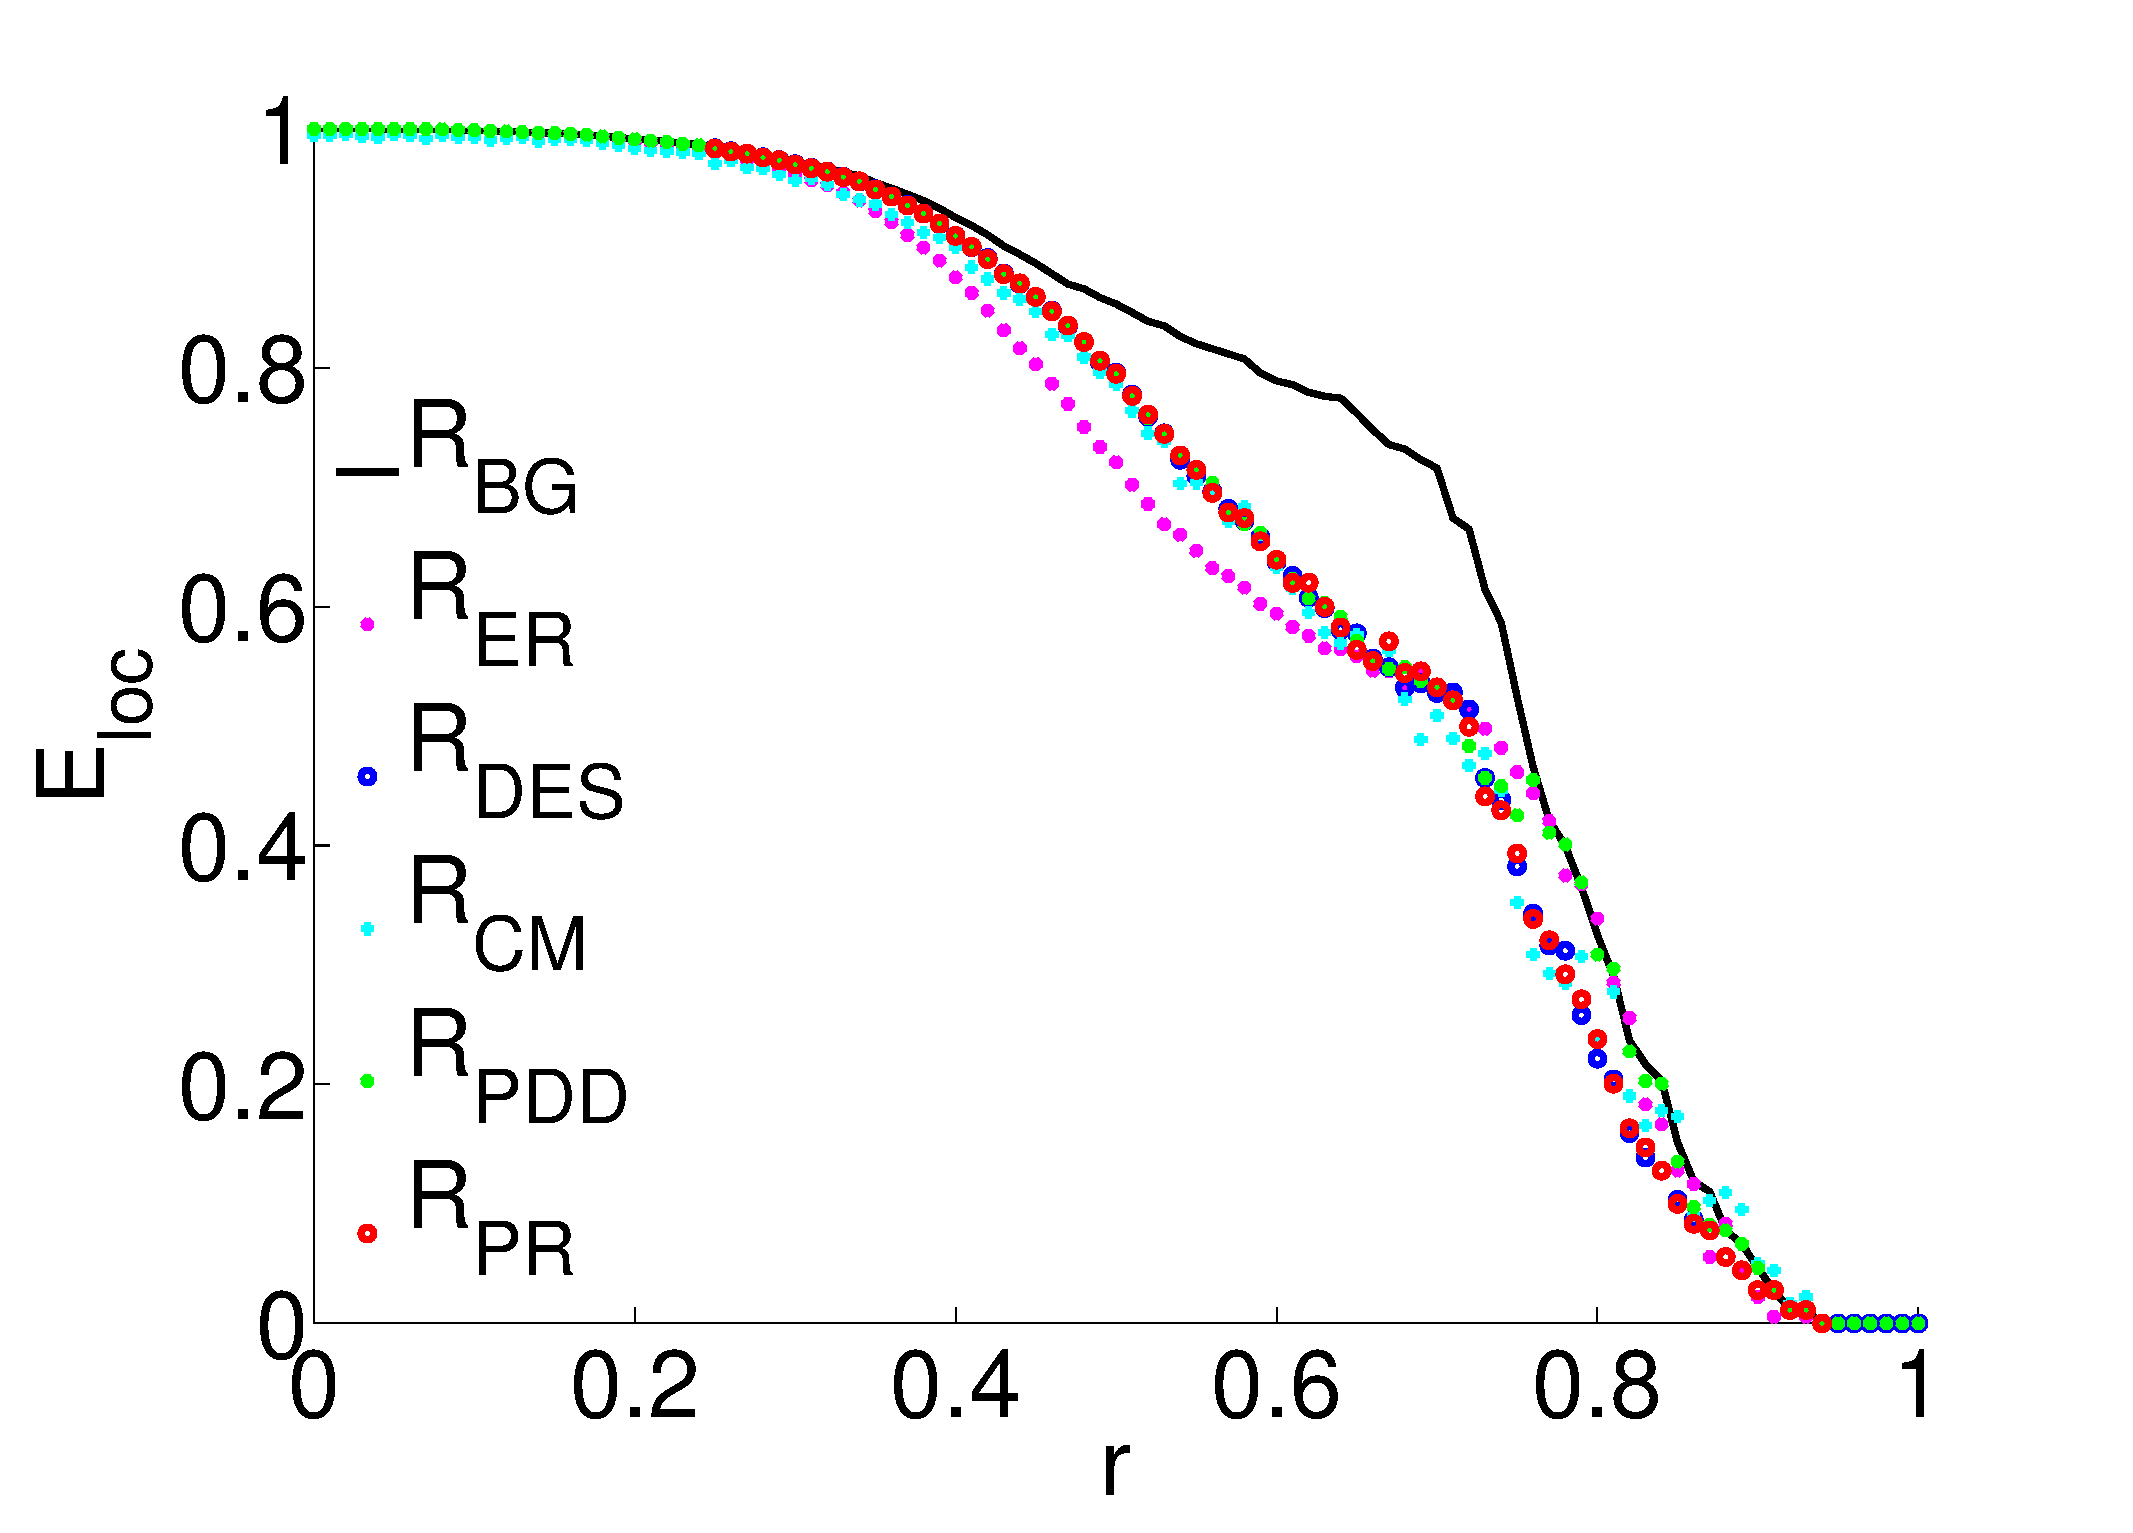
\includegraphics[width=0.49\textwidth]{Figures/Local_Efficiency_Average_Fnc.eps}
	 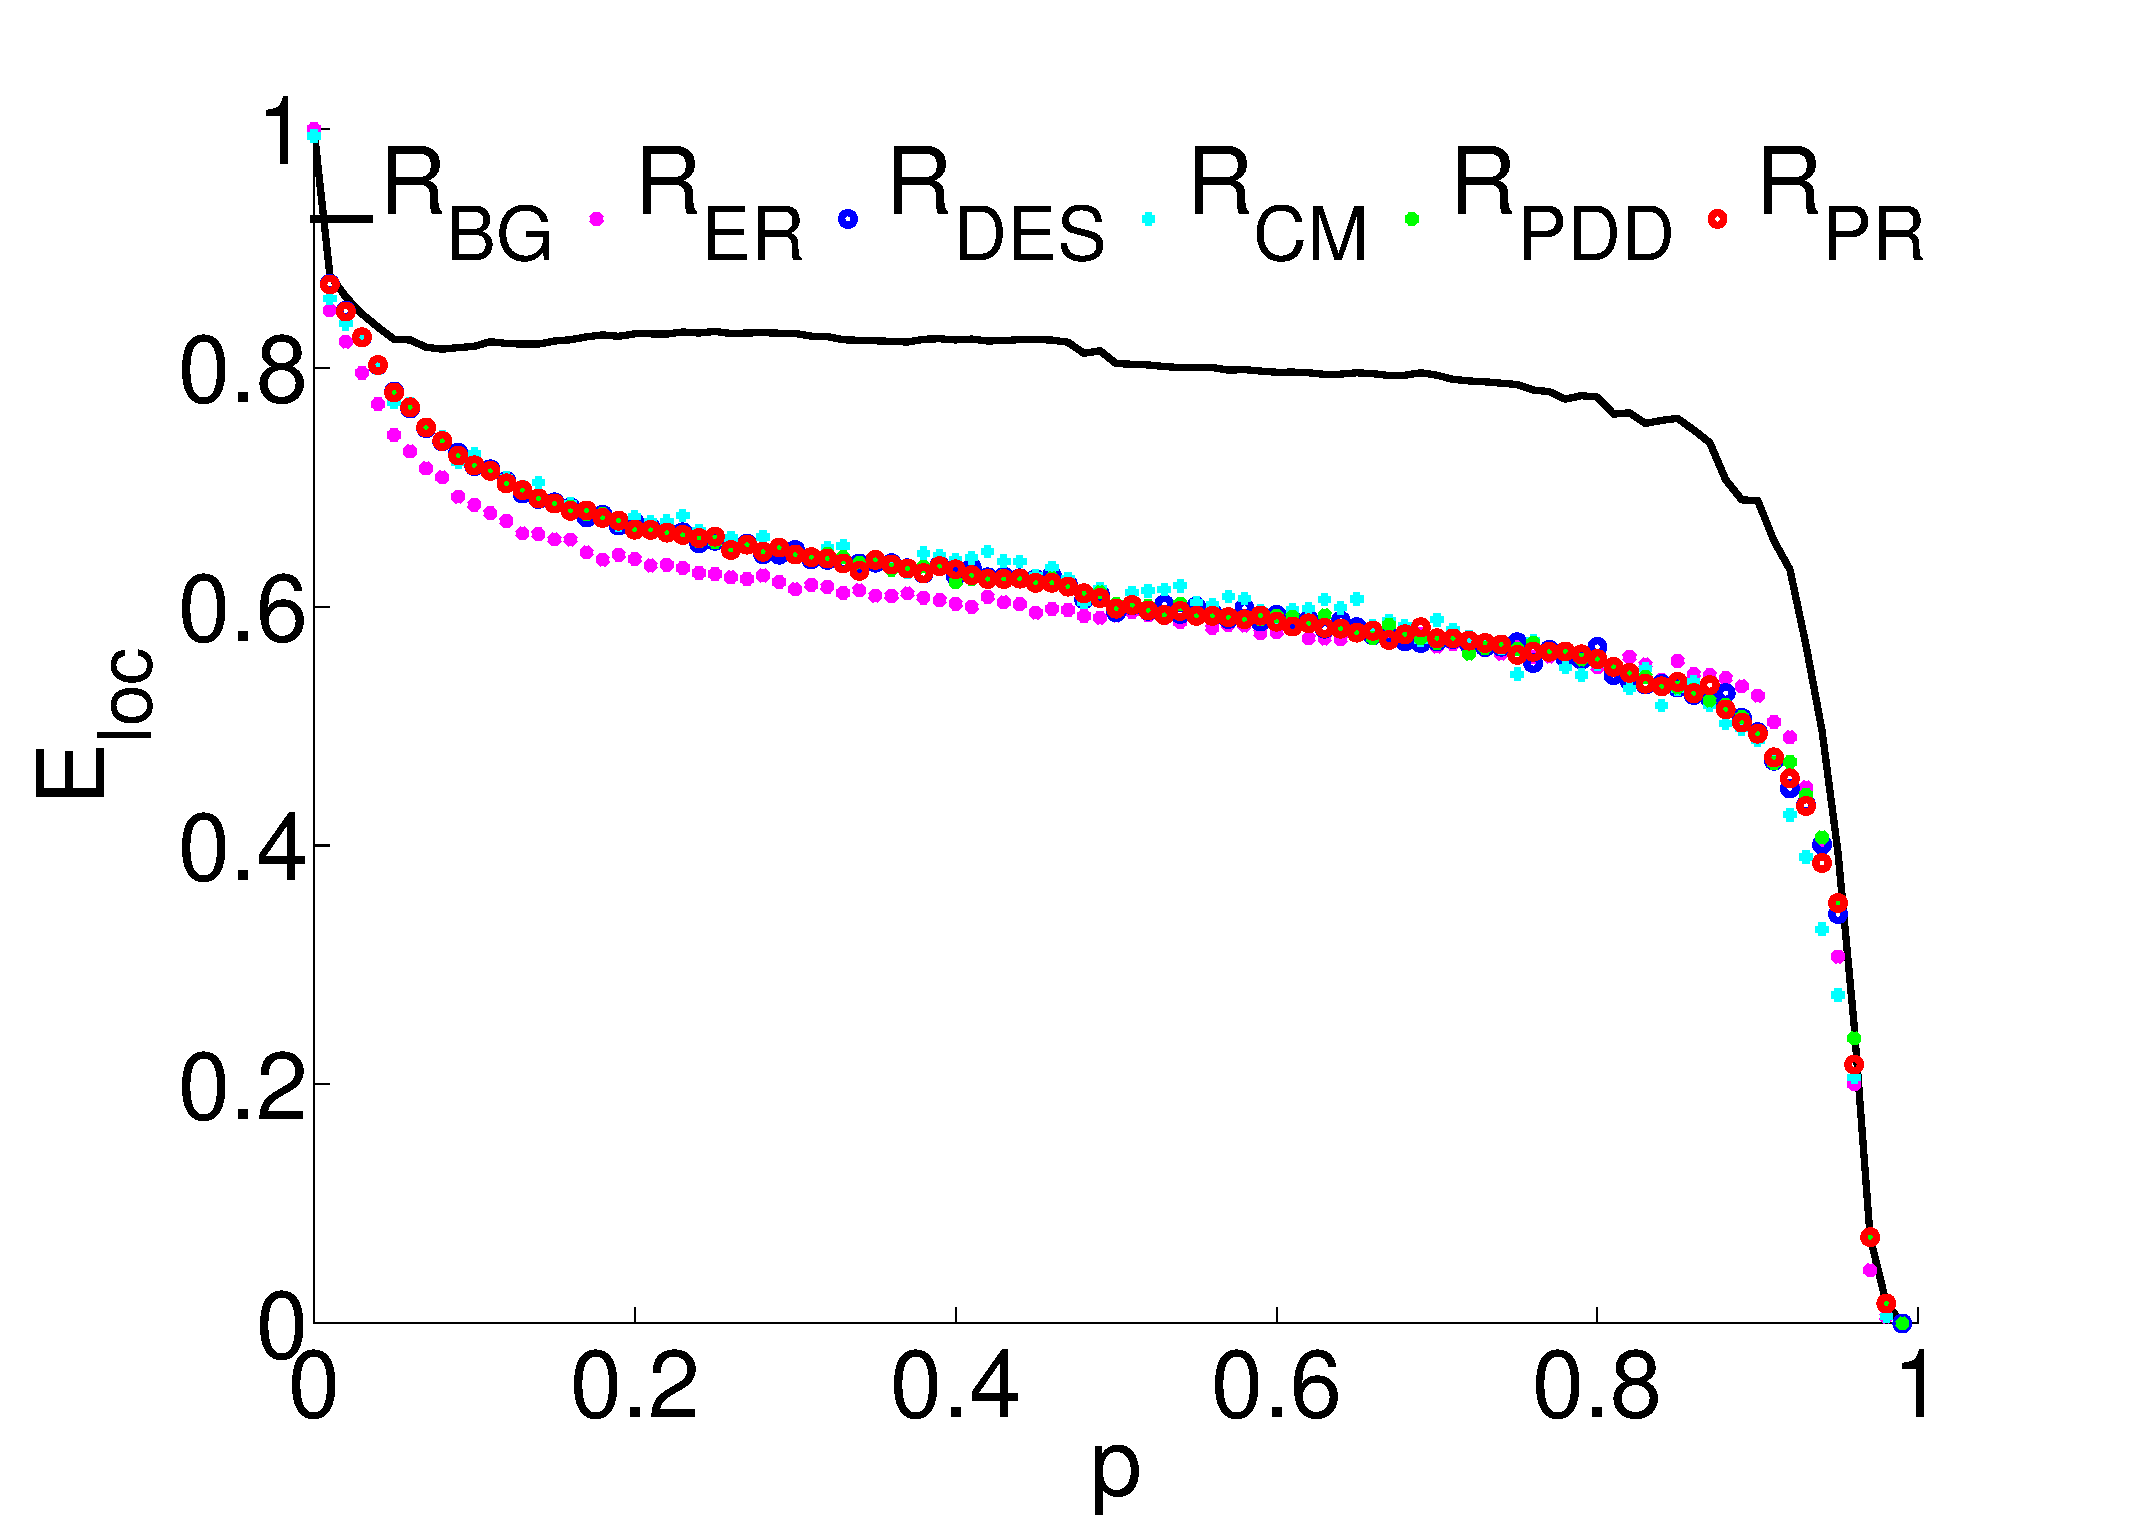
\includegraphics[width=0.49\textwidth]{Figures/Local_Efficiency_Average_Stru.eps}
	\rule{35em}{0.5pt}  
  \caption[Local Efficiency]{$E_{loc}$ of the functional connectivity map derived $R_{BG}$ and its randomized networks on the left and $E_{loc}$ of the anatomical map derived $R_{BG}$ and its randomized networks on the right. } 
    \label{fig:Local Efficiency}
 	
\end{figure}

Brain graphs based on FCM and ACM tend to have higher $E_{loc}$ than their random graphs. Anatomical connectivity matrix related networks have in general higher $E_{loc}$ compared to the functional connectivity matrix related networks. Local information transmit is more efficient in ACM than in FCM. The graphs with larger $E$ compared to the $R_{BG}$ in Figure B.3 exhibit lower $E_{loc}$ in Figure B.4.   


\section{Small Worldness}

A small world network is both highly segregated and integrated, a measure of small worldness $S$ was proposed to capture this effect in a single statistic,

\begin{equation}
S = \frac{C/C_{rand}}{L/L_{rand}} \,\, ,
\end{equation}
 
where $C$ and $C_{rand}$ are clustering coefficients, $L$ and $L_{rand}$ are characteristic path lengths of the original and random network respectively \citep{HUM08}. The random network here is constructed with \textit{Erd\H{o}s-R\'{e}nyi} method, which has the same number of nodes and links as the reference graph:

\begin{equation}
L = \frac{1}{n}\sum\limits_{i \epsilon N} L_i = \frac{1}{n}\sum\limits_{i \epsilon N} \frac{\sum\limits_{j \epsilon N, j \neq i }d_{ij}}{n-1 } \,\, .
\end{equation}


\begin{figure}[htbp]
 
  \centering
	 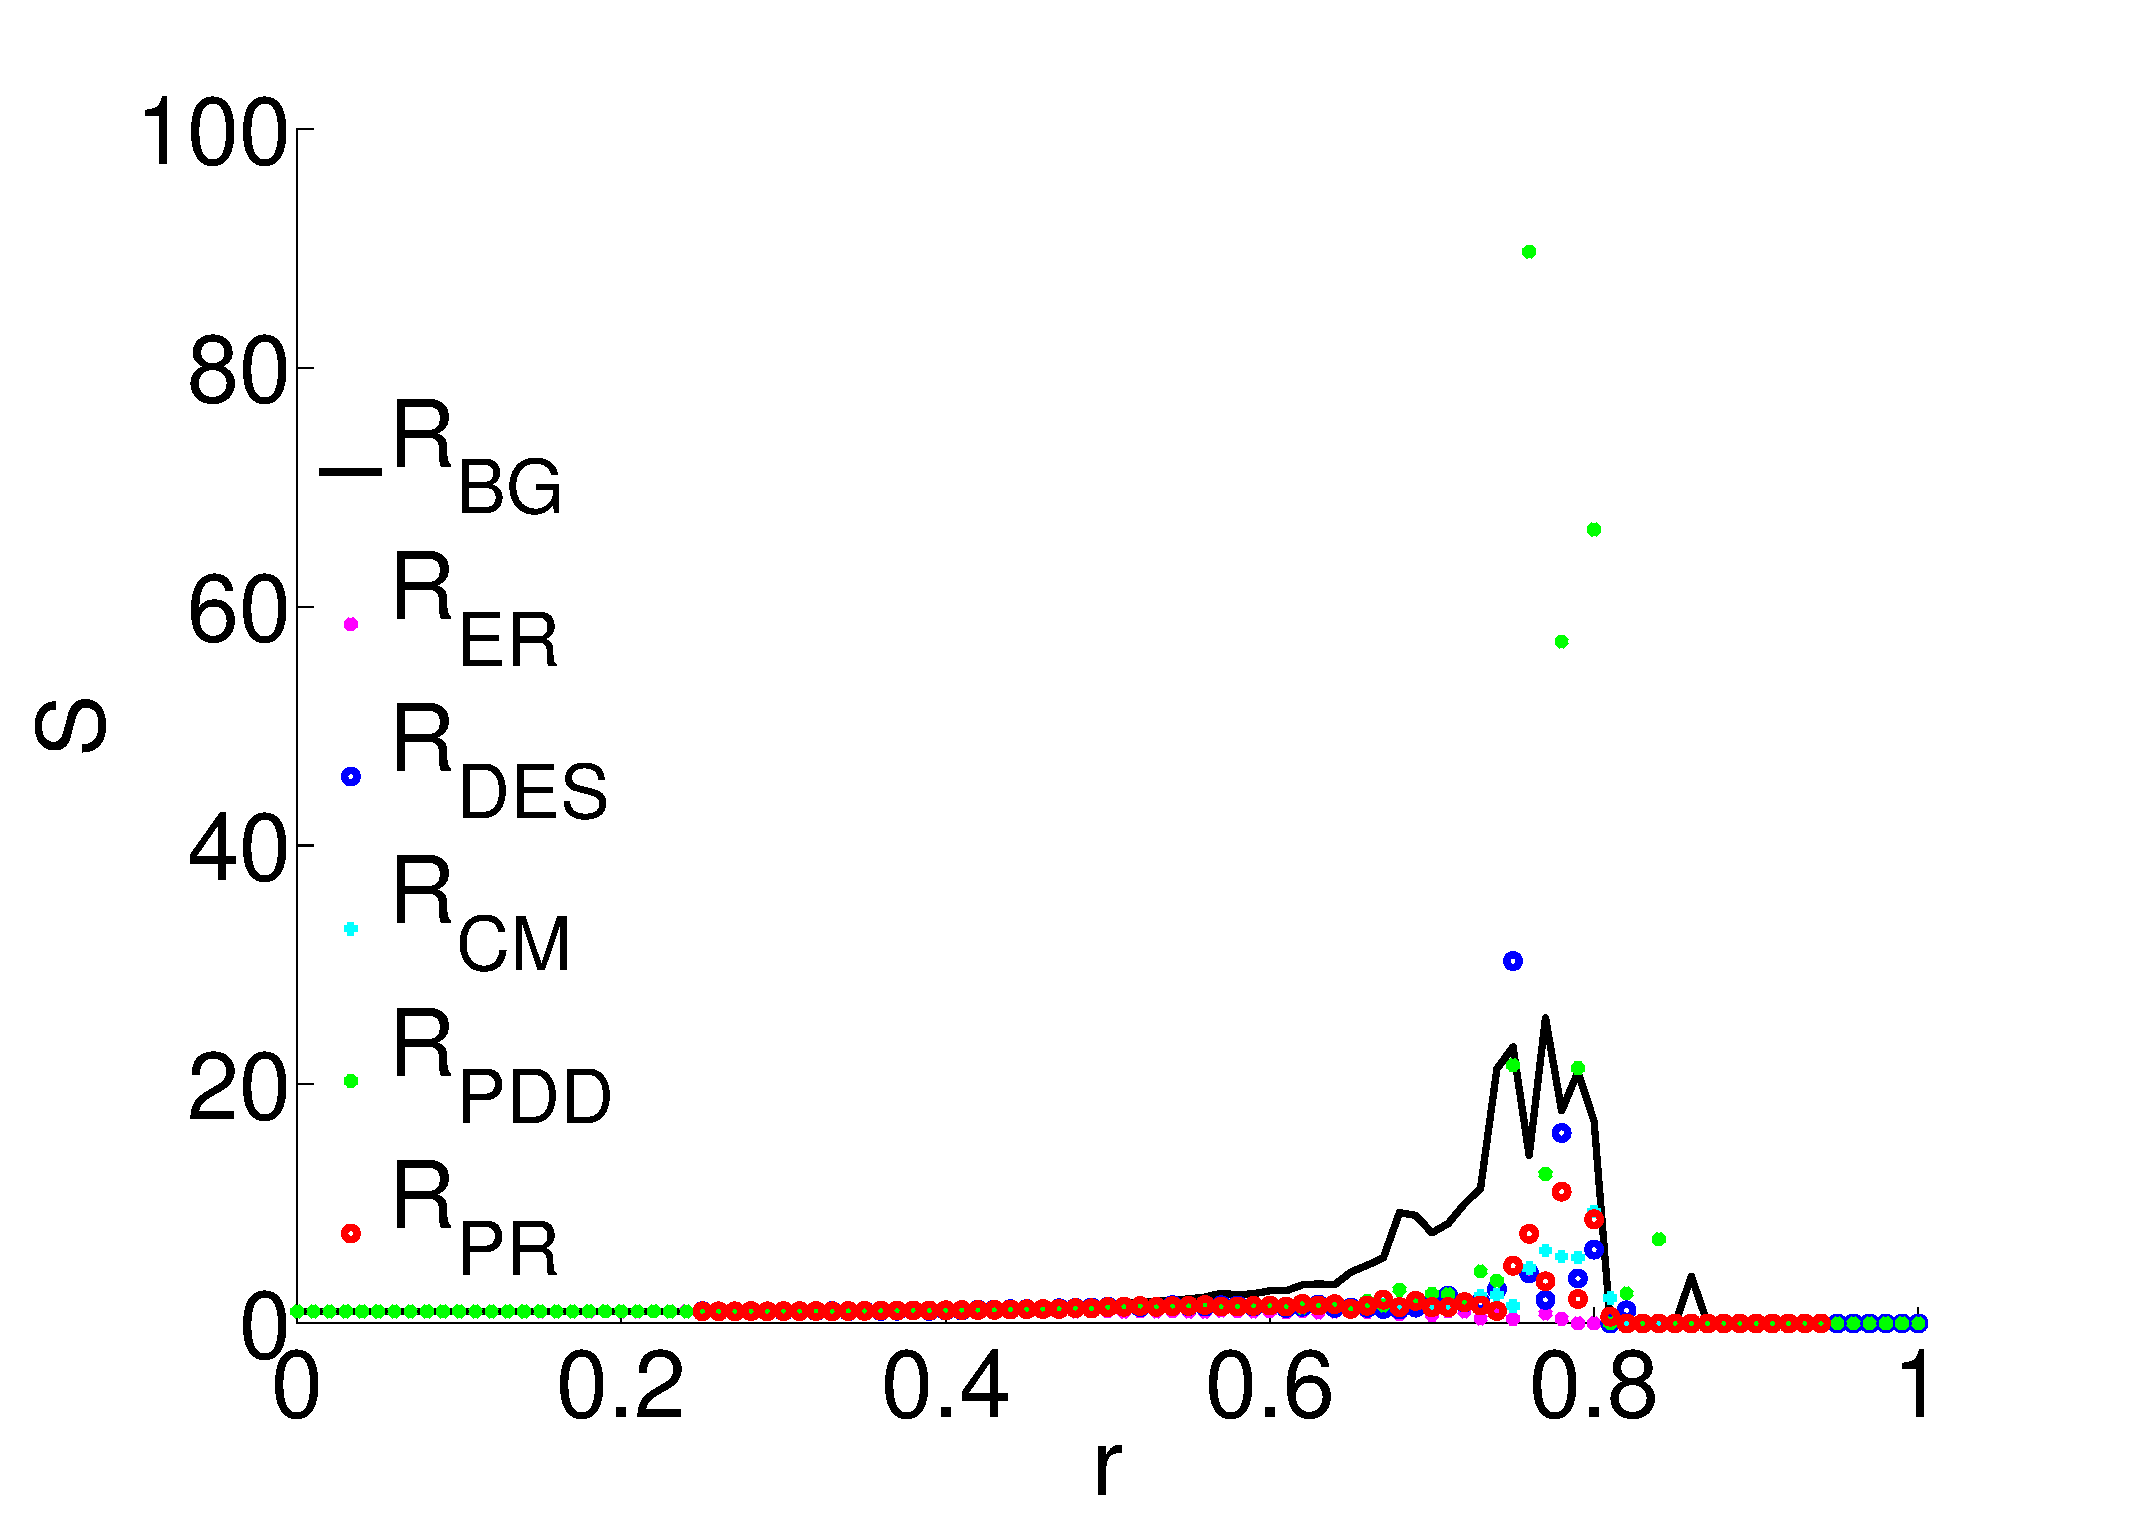
\includegraphics[width=0.49\textwidth]{Figures/Small_Worldness_Fnc.eps}
	 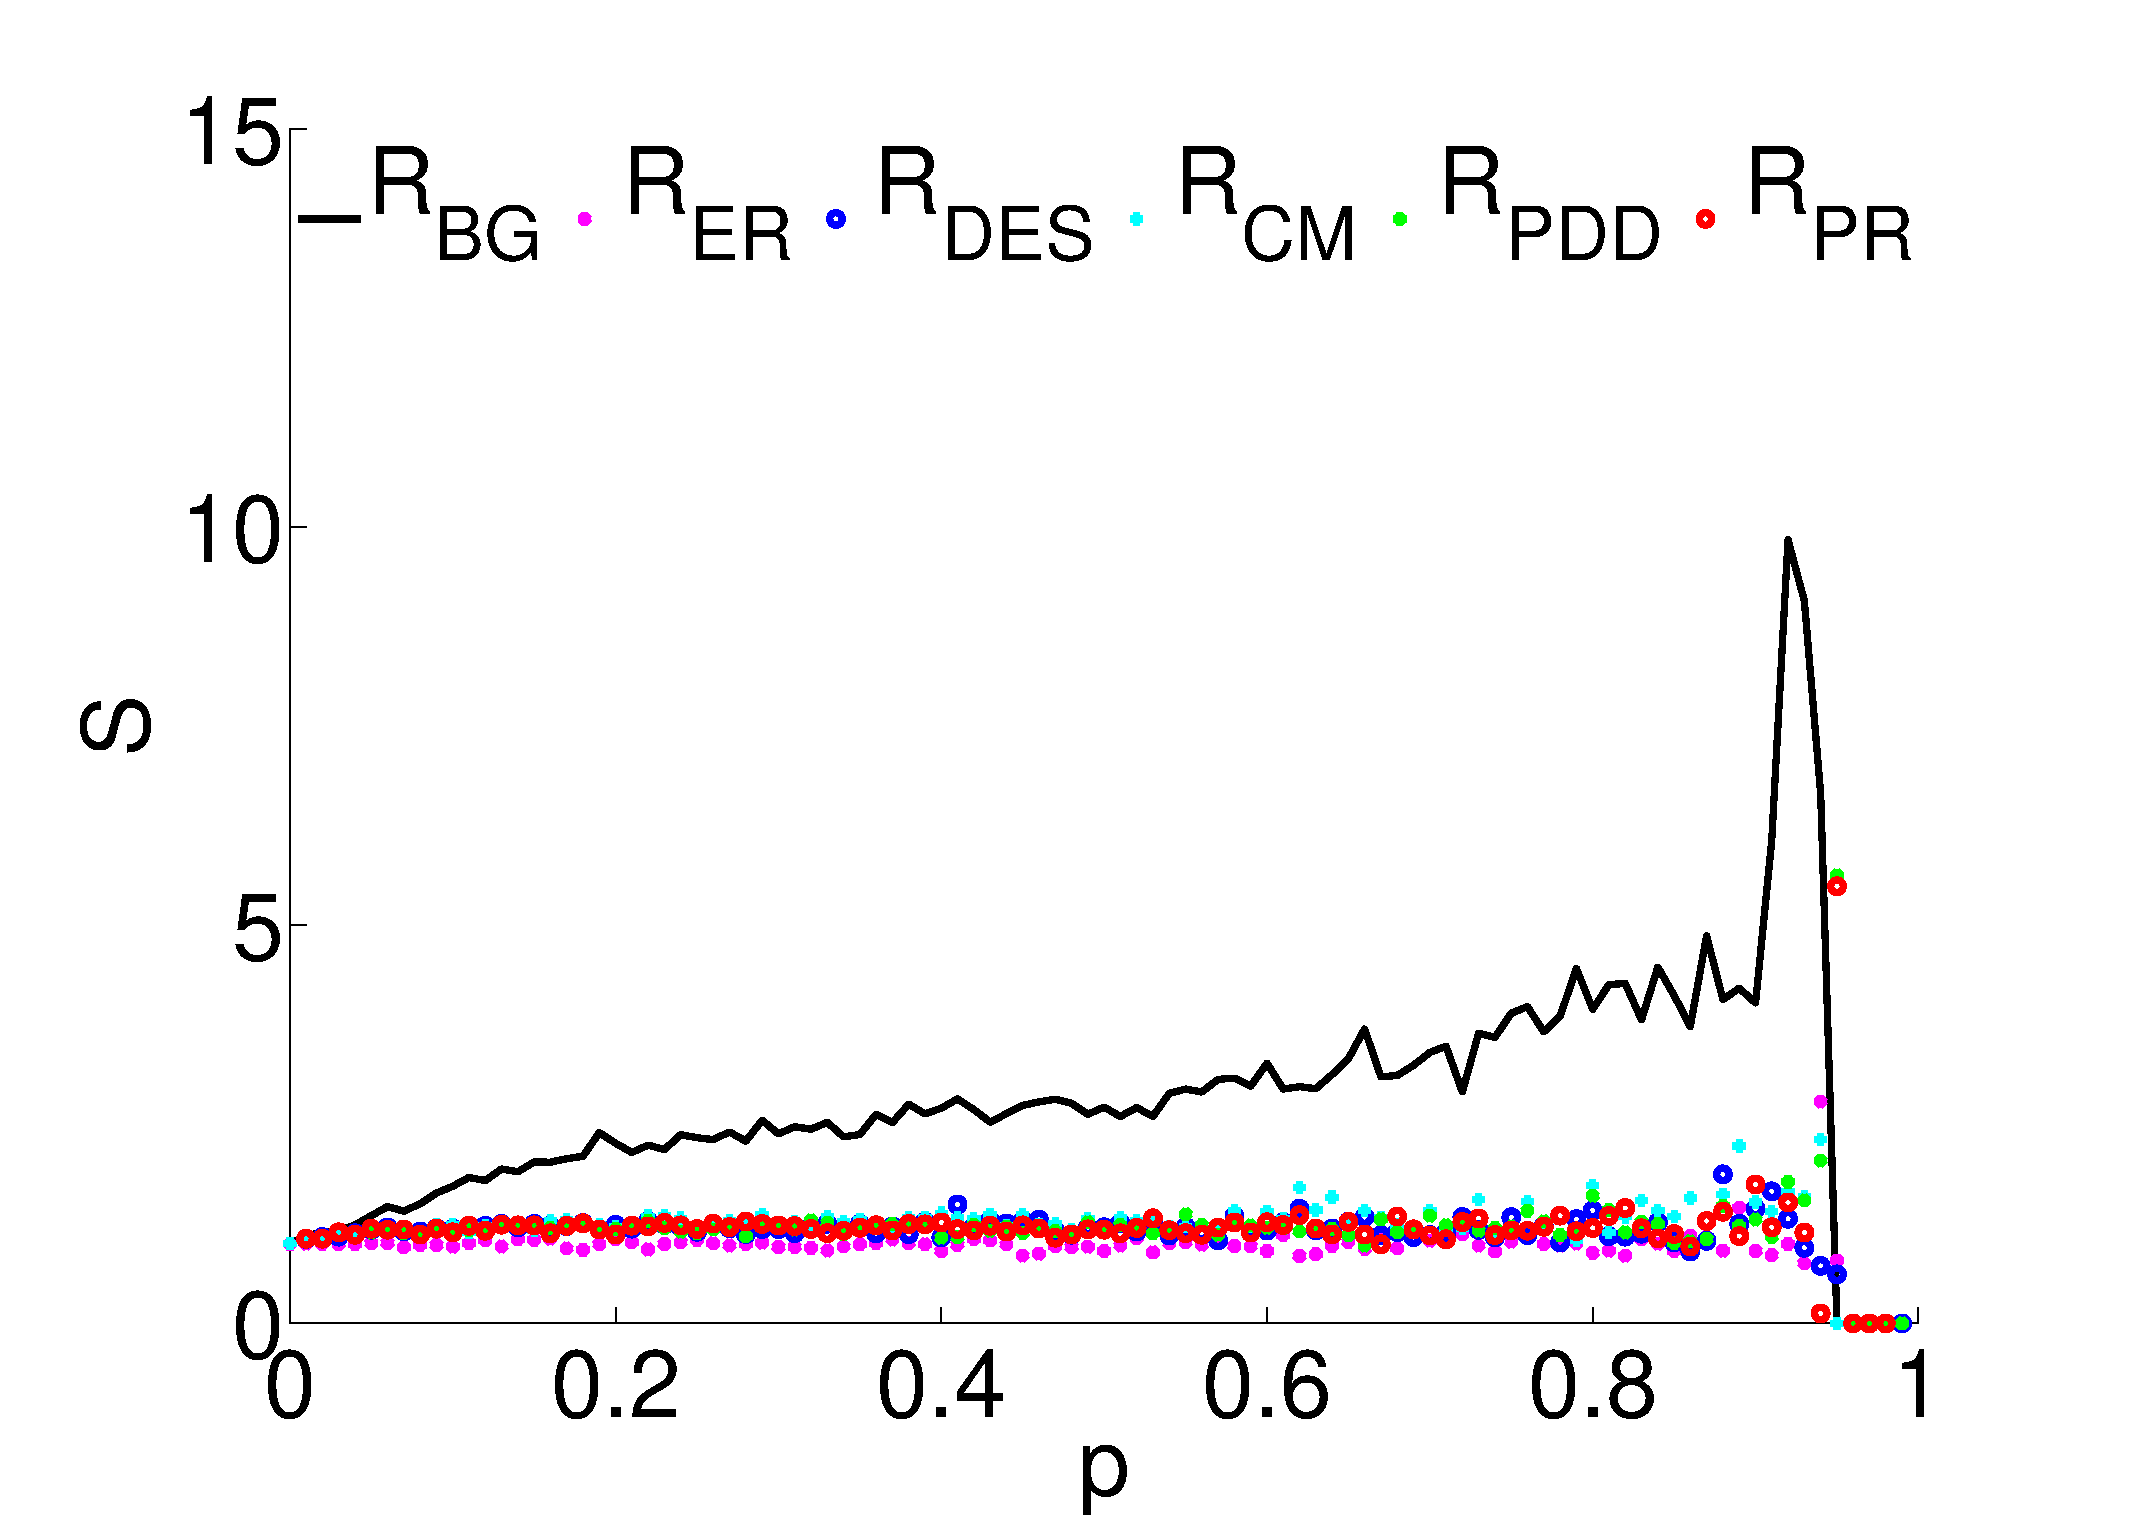
\includegraphics[width=0.49\textwidth]{Figures/Small_Worldness_Stru.eps}
	\rule{35em}{0.5pt}
  \caption[Small Worldness]{Small worldness of the anatomical (left) and functional (right) brain graphs and their random graphs.} 
    \label{fig:Small Worldness}
 	
\end{figure}


In Figure B.5, brain graphs have higher $S$ than random graphs for both FCM and ACM. In comparison to other network measurements up to here, $S$ measure makes brain graphs the most distinguishable than random graphs. At some unique $r$ and $p$ values, random graphs $R_{DES}$, $R_{PDD}$ (left) and $R_{PDD}$, $R_{PR}$ (right) tend to have quite large $S$. However, this does not change the general high $S$ pattern of brain graphs. Random networks seem to be equally segregated and integrated in general, but the real networks behave differently. 



\section{Assortativity}

Assortativity measures the correlation coefficient between the degrees of all nodes on two opposite ends of a link \citep{RUB10}. Assortativity coefficient $A$ of a network is given by the following equation; 

\begin{equation}
A = \frac{\dfrac{1}{l} \sum\limits_{(i,j) \in L}  k_i k_j -  \Big ( \dfrac{1}{2L} \sum\limits_{(i,j) \in L}k_i + k_j  \Big )^2}{\dfrac{1}{2L}\sum\limits_{(i,j) \in L} ( k_i^2+  k_j^2) -\Big ( \dfrac{1}{2L} \sum\limits_{(i,j) \in L}k_i + k_j  \Big )^2 } \,\, ,
\end{equation}

where $L$ is number of edges in, $k_i$ is degree of node $i$ \citep{NEW02a}.


\begin{figure}[htbp]
 
  \centering
	 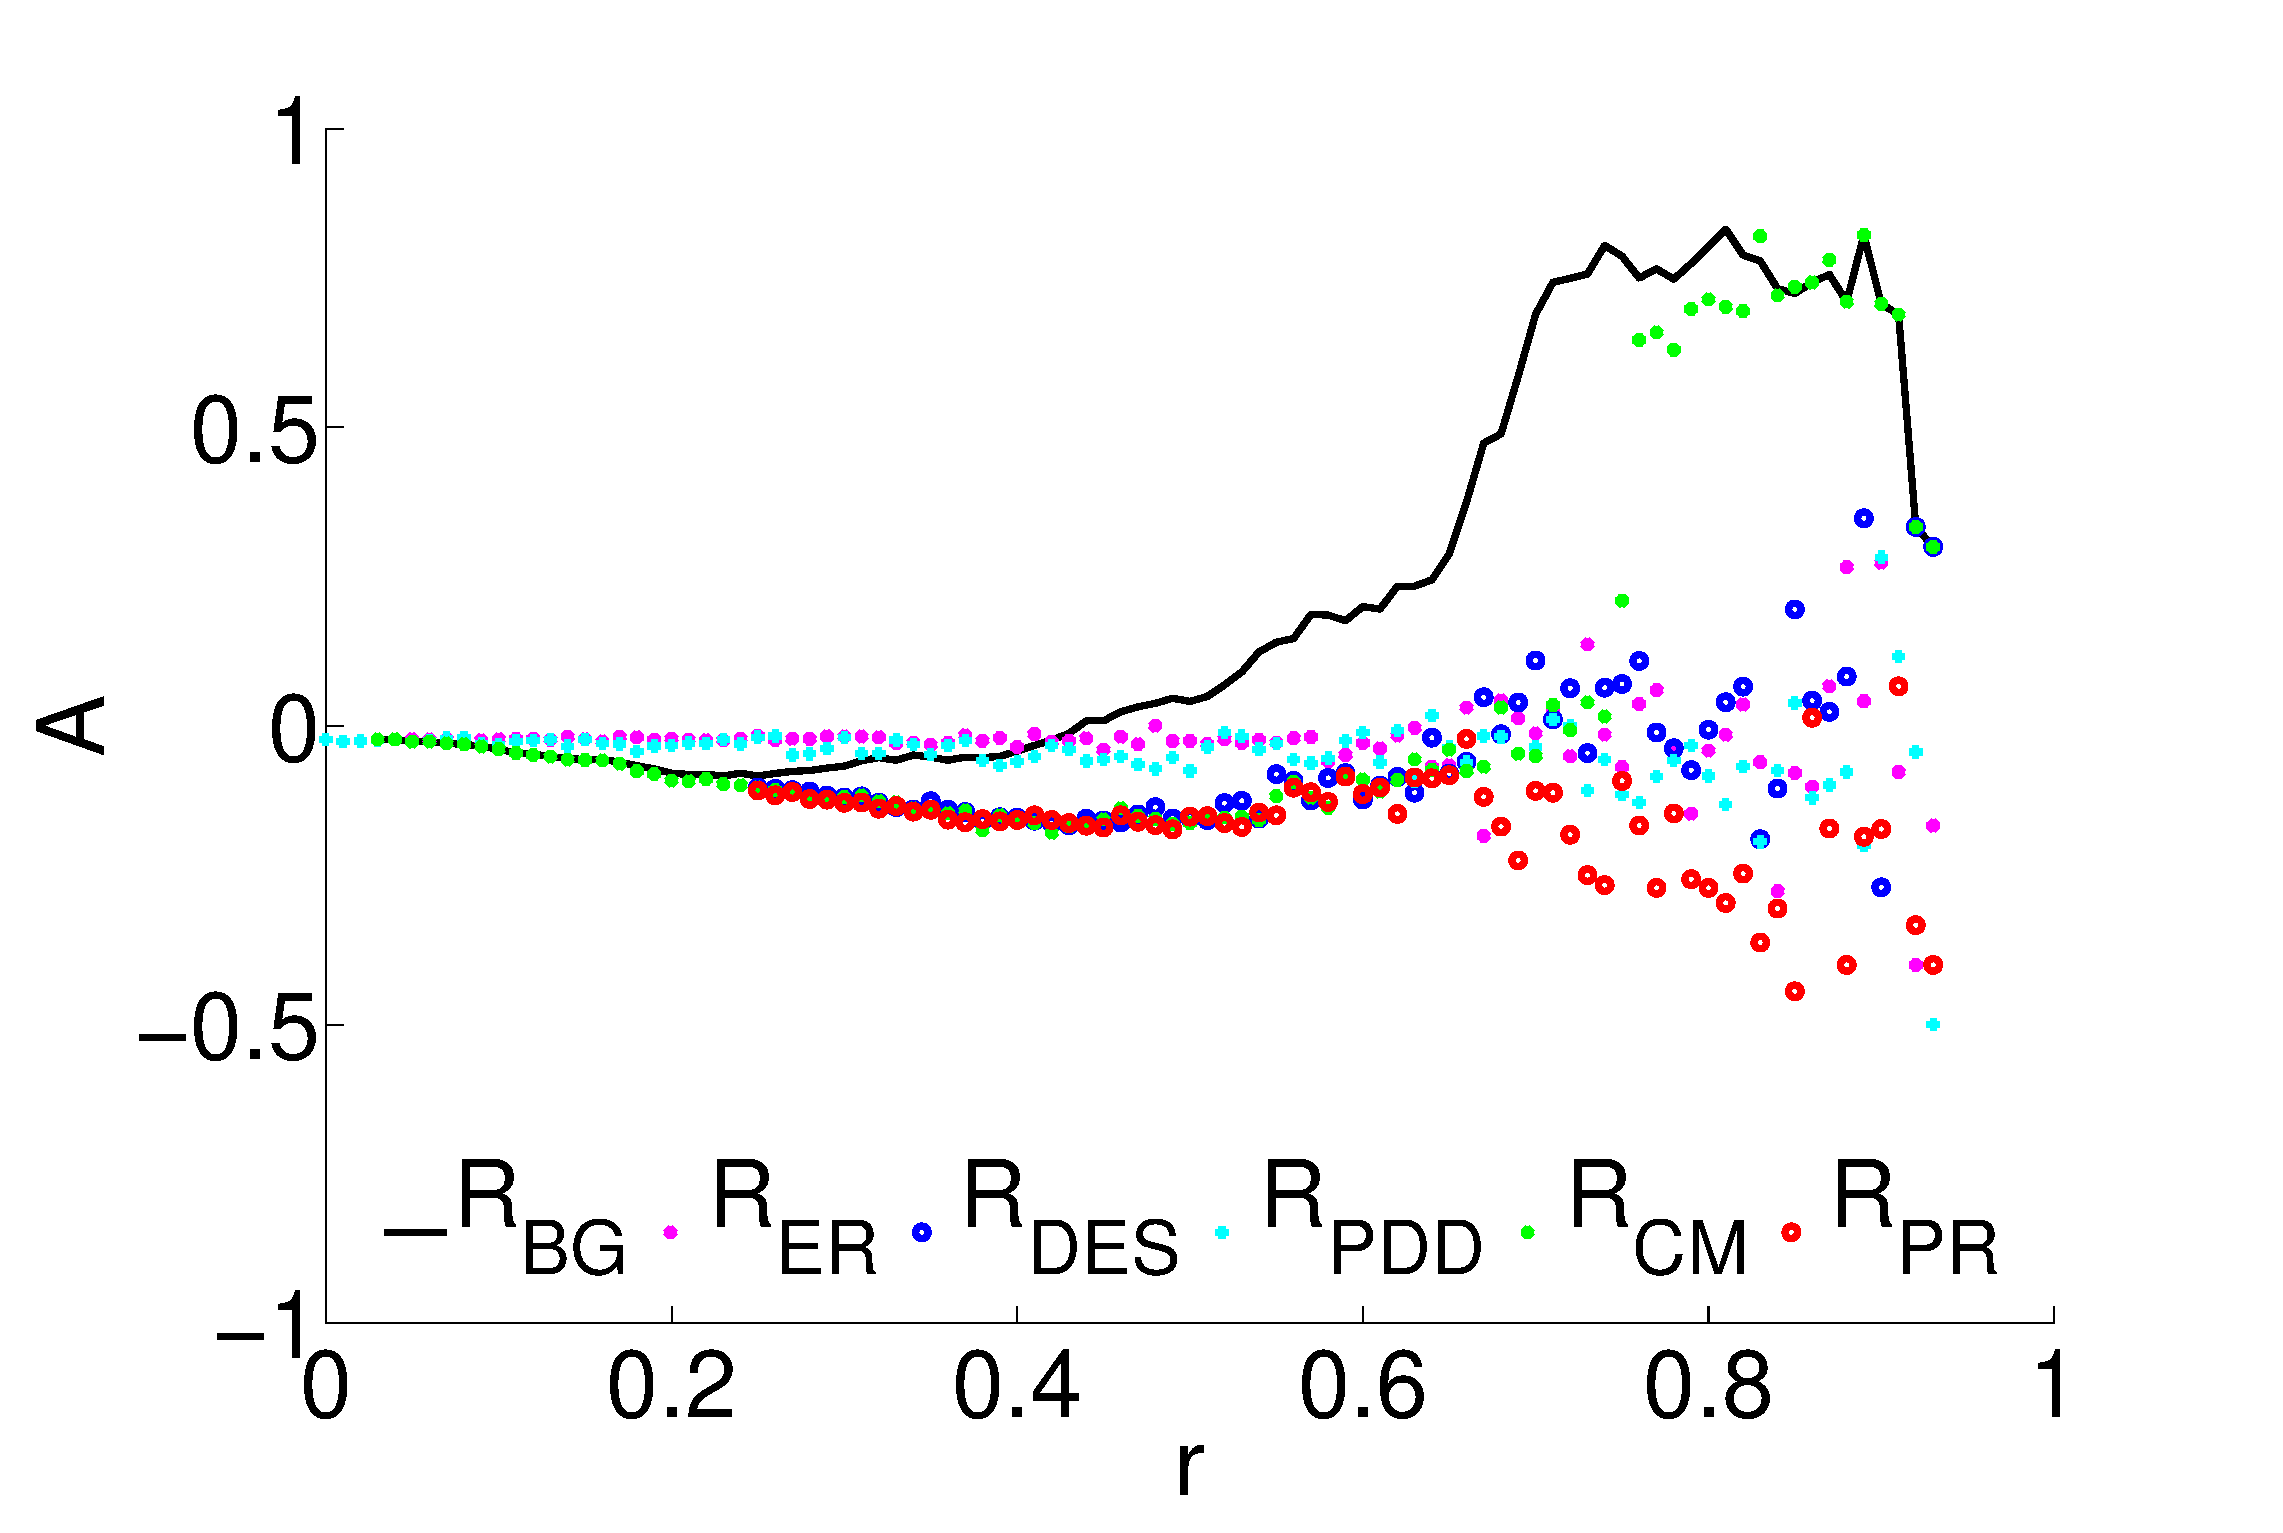
\includegraphics[width=0.49\textwidth]{Figures/Assortativity_Fnc.eps}
	 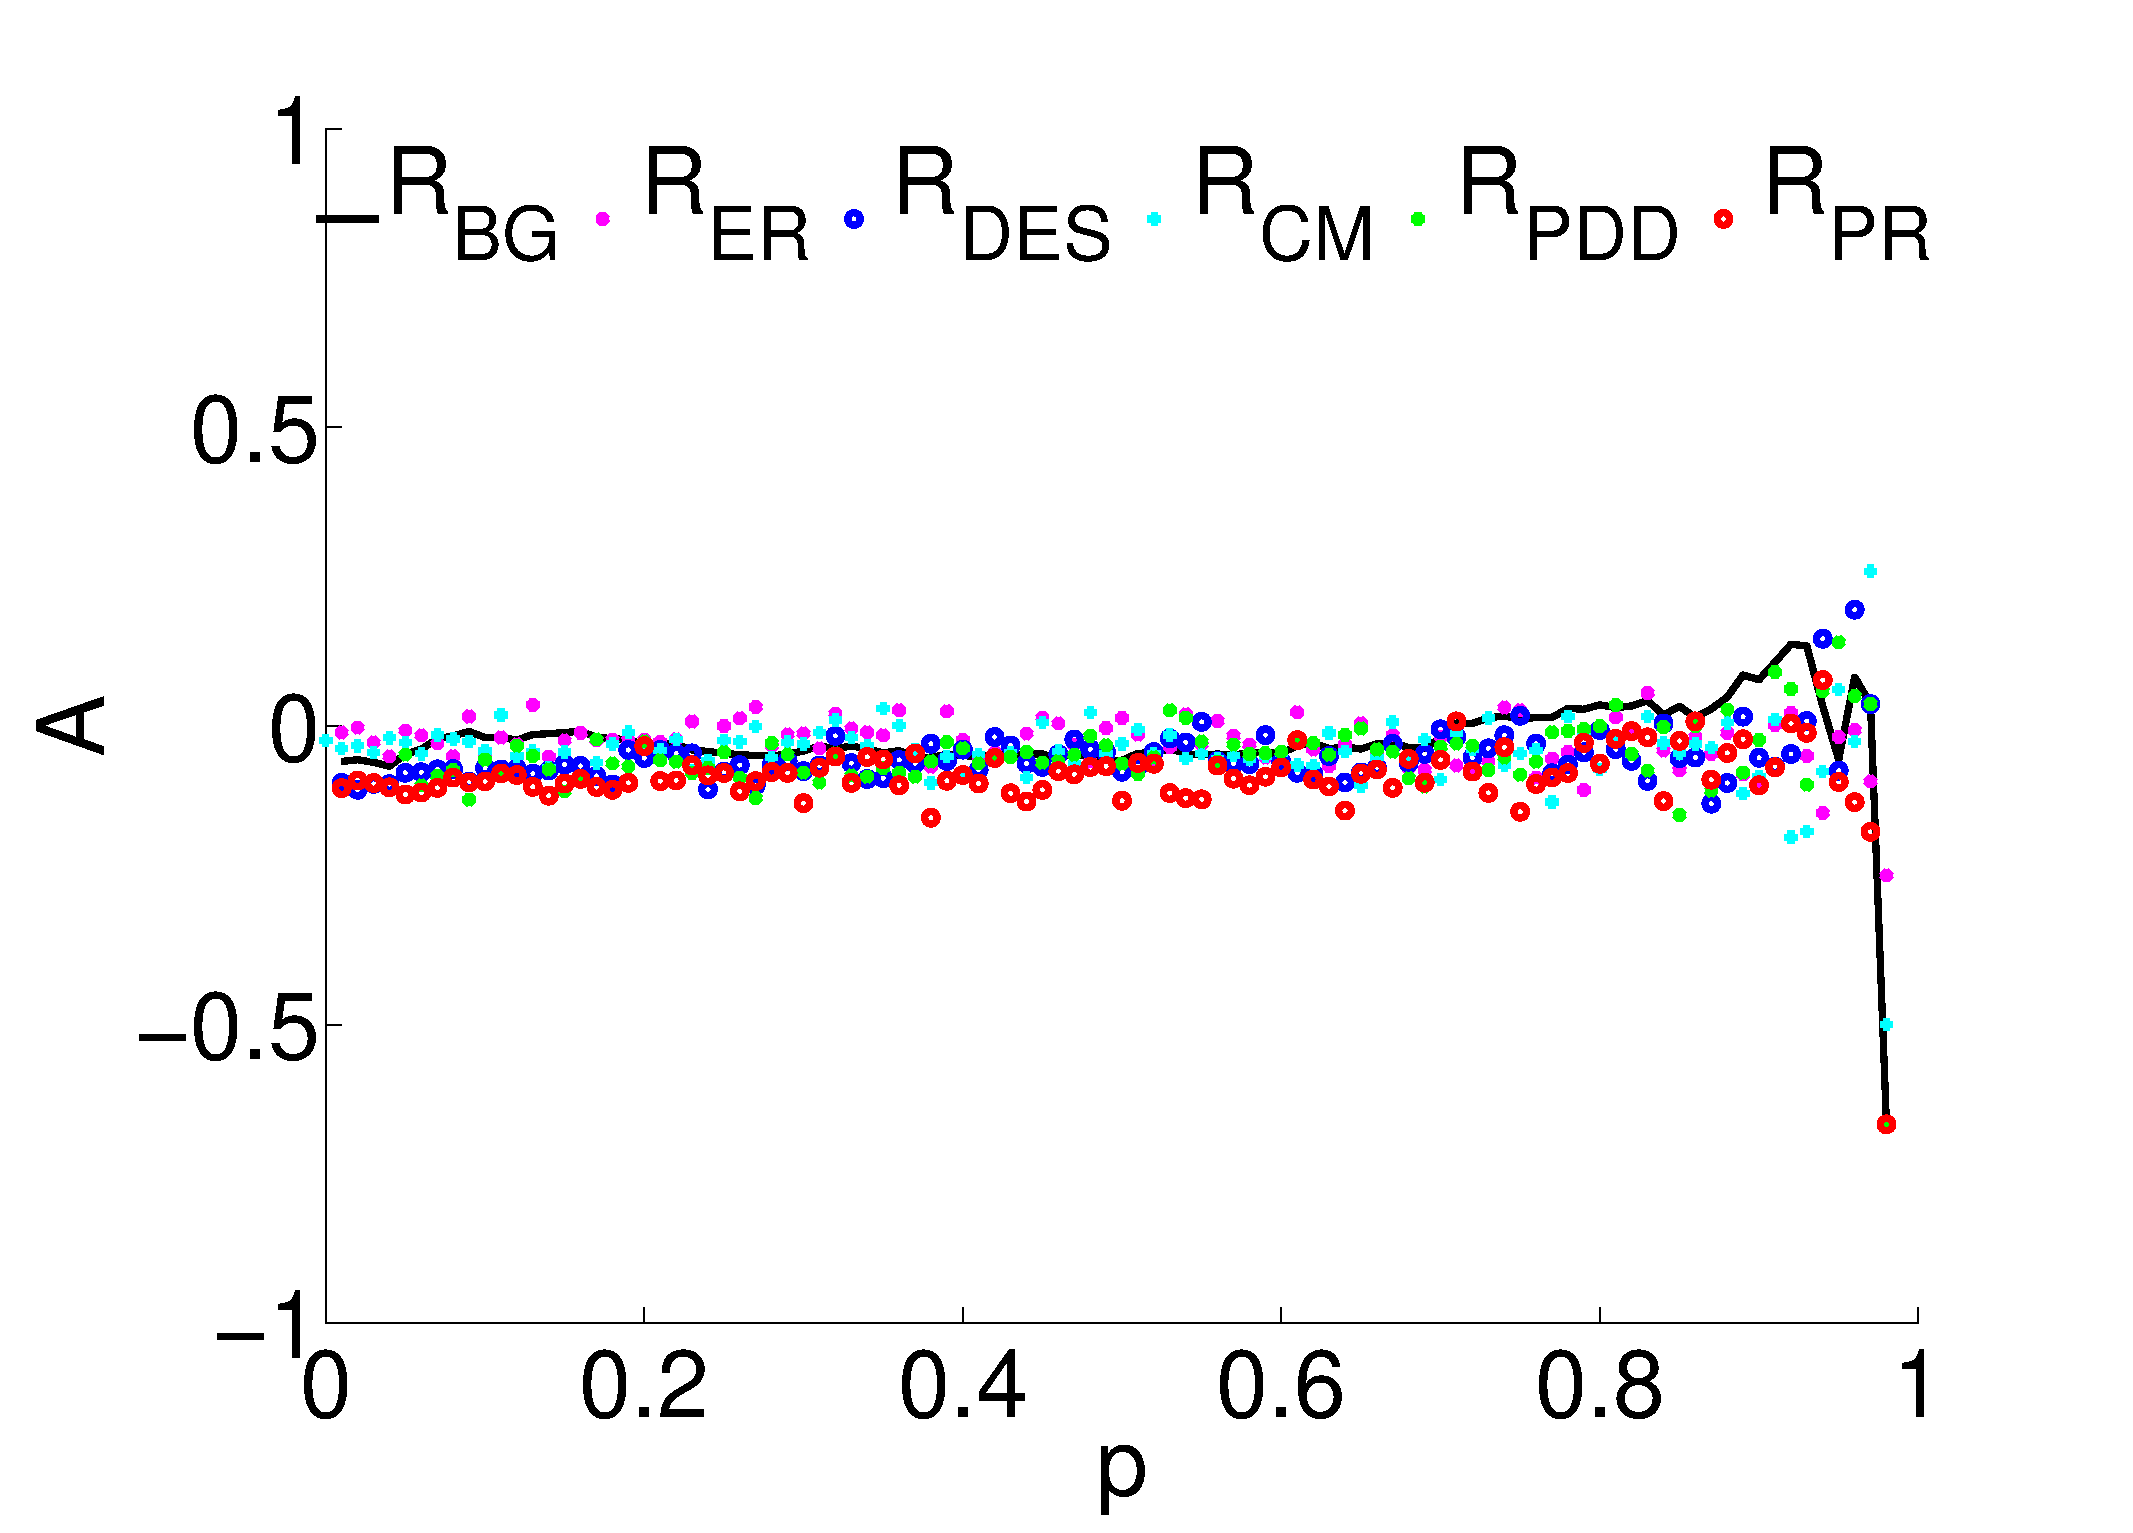
\includegraphics[width=0.49\textwidth]{Figures/Assortativity_Stru.eps}
    \rule{35em}{0.5pt}
  \caption[Assortativity]{Assortativity coefficients of FCM (left) and ACM (right) brain graphs and their random graphs.} 
    \label{fig:Assortativity}
 	
\end{figure}

Negative assortativity presents a network having widely distributed high-degree hubs \citep{RUB10}. On the other hand, assortativity coefficients close to $1$ indicates a graph having fine correlated degree nodes. $A$-values follow a very similar pattern around 0 for all the graphs based on ACM as seen in Figure B.6. The degrees of nodes seem not to be significantly correlated. However, $A$-values of FCM related networks are more diverse. The degrees of nodes are highly correlated in FCM brain graph, particularly at large $r$, whereas random graphs exhibit anti-correlations among node degrees.   

\section{Average Connected Components}
The connected components of an indirected graph indicates the number of subgraphs in overall network. Subgraph can be imagined as a connected group of nodes which have globally no connection to any other subgraph. In order to visualize subgraphs algebraically, let us define number of edges $L$ of graph $G$ in terms of three subgraphs of $G$:
\begin{equation}
L_G = L_{G_1}\cup L_{G_2}\cup L_{G_3} . 
\end{equation} 

\begin{figure}[htbp]
 
  \centering
	 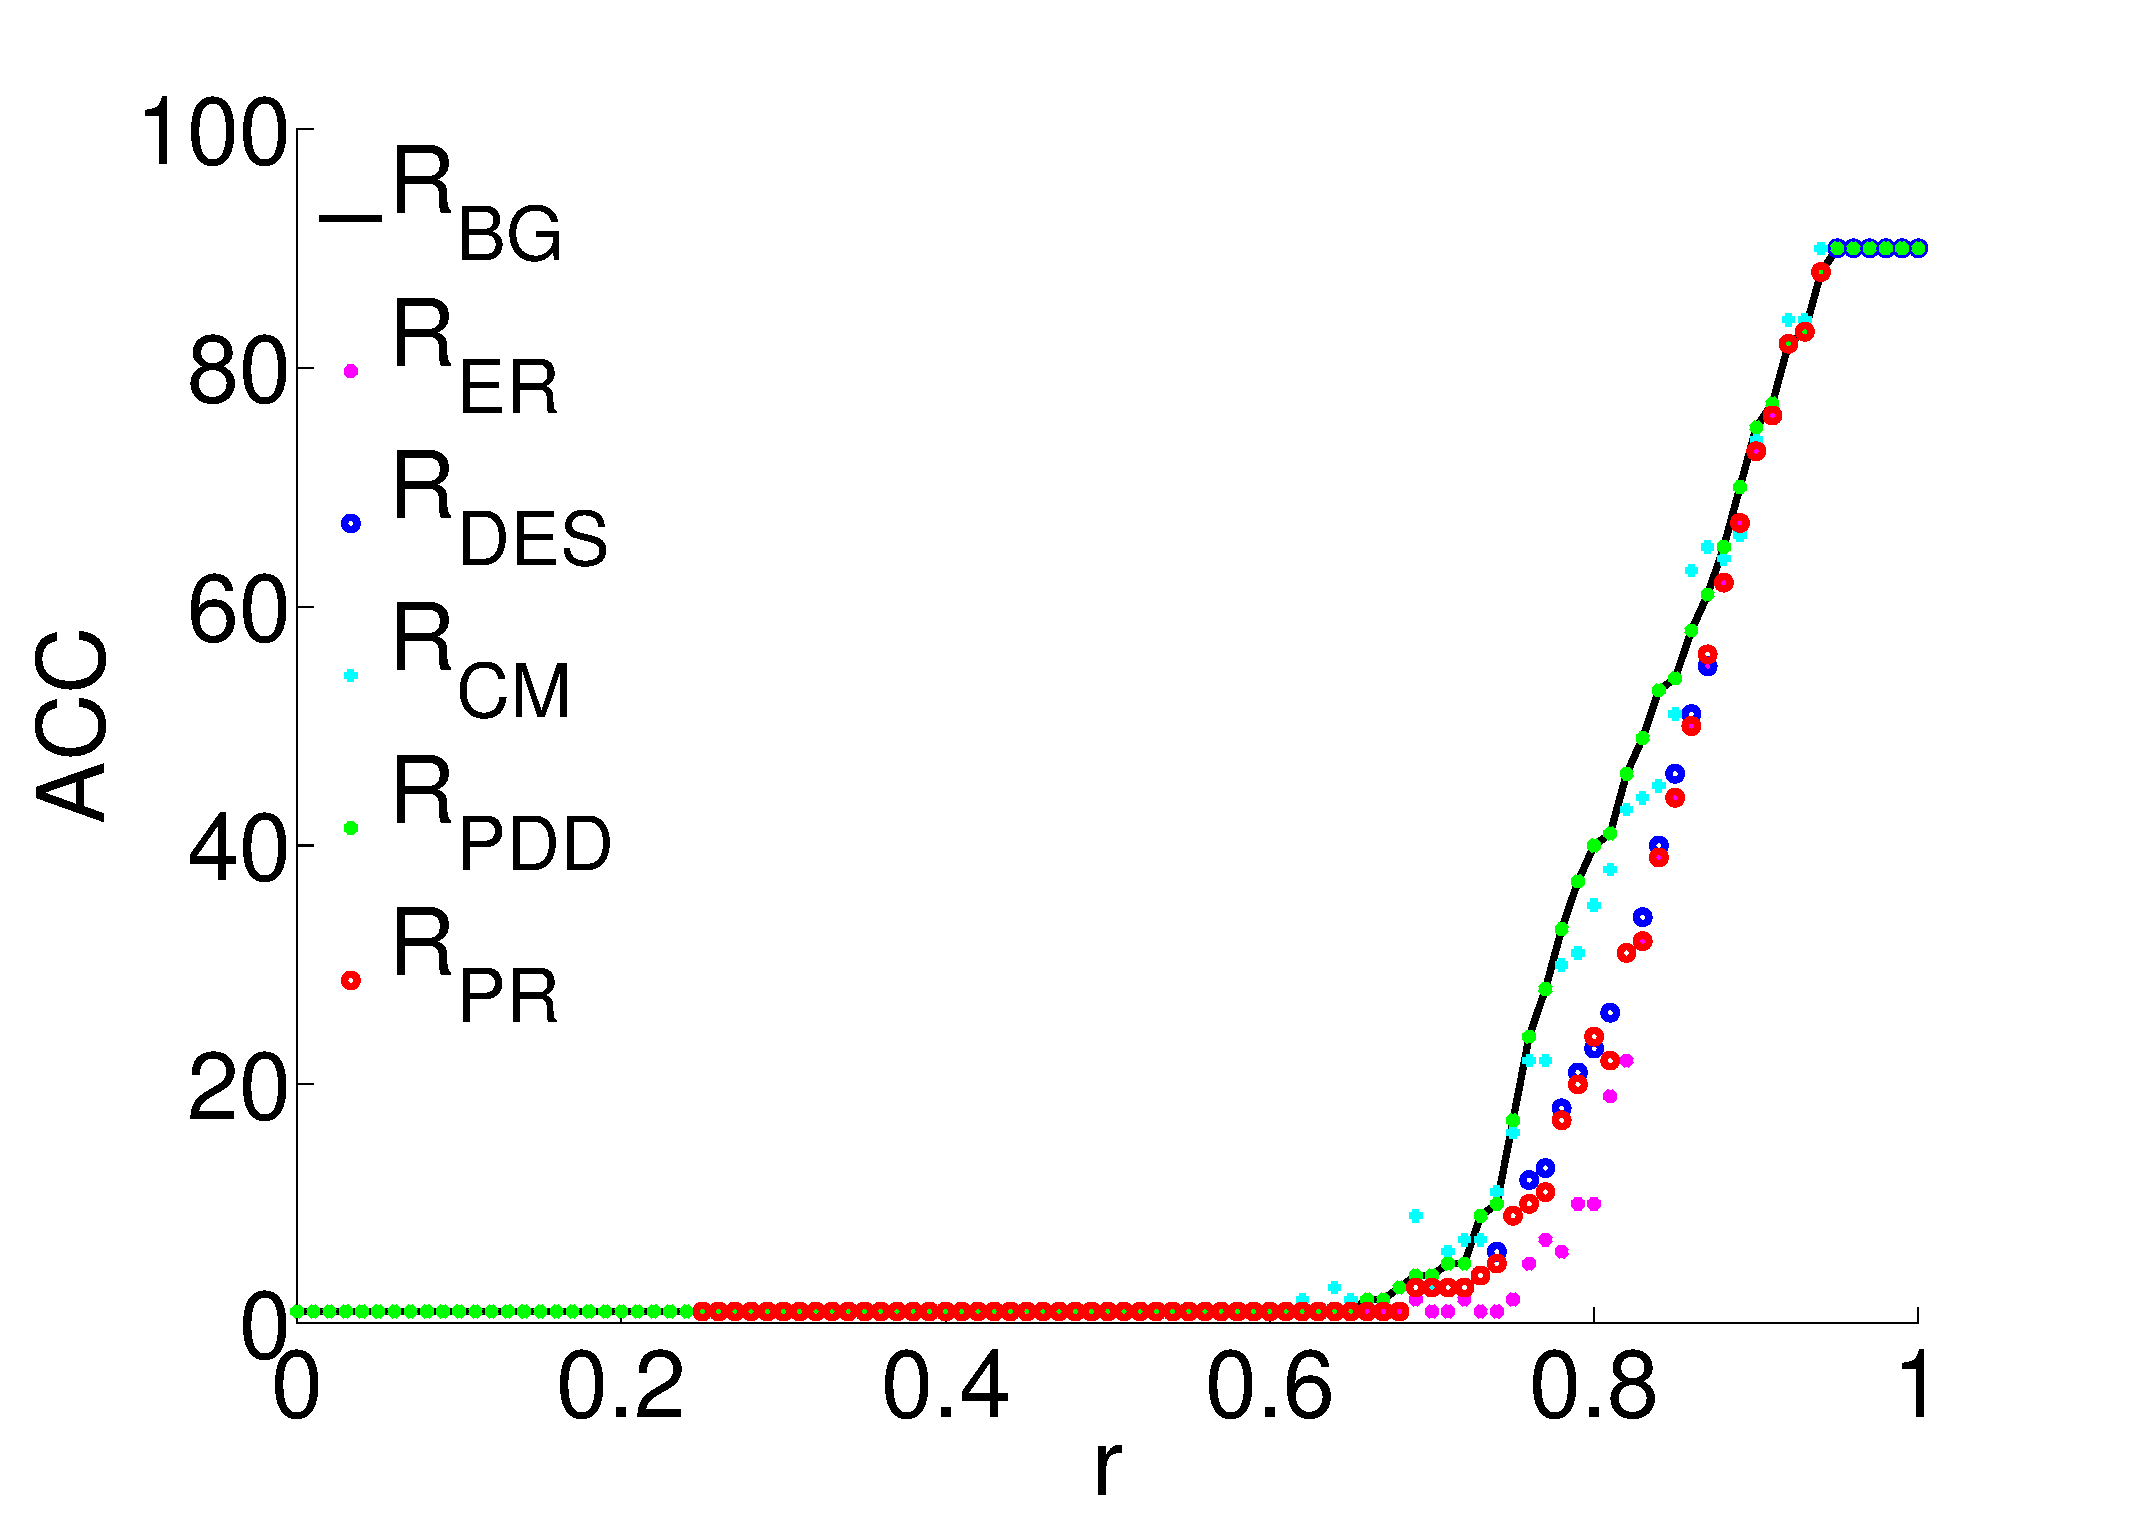
\includegraphics[width=0.49\textwidth]{Figures/connec_compo_FCM.eps}
	 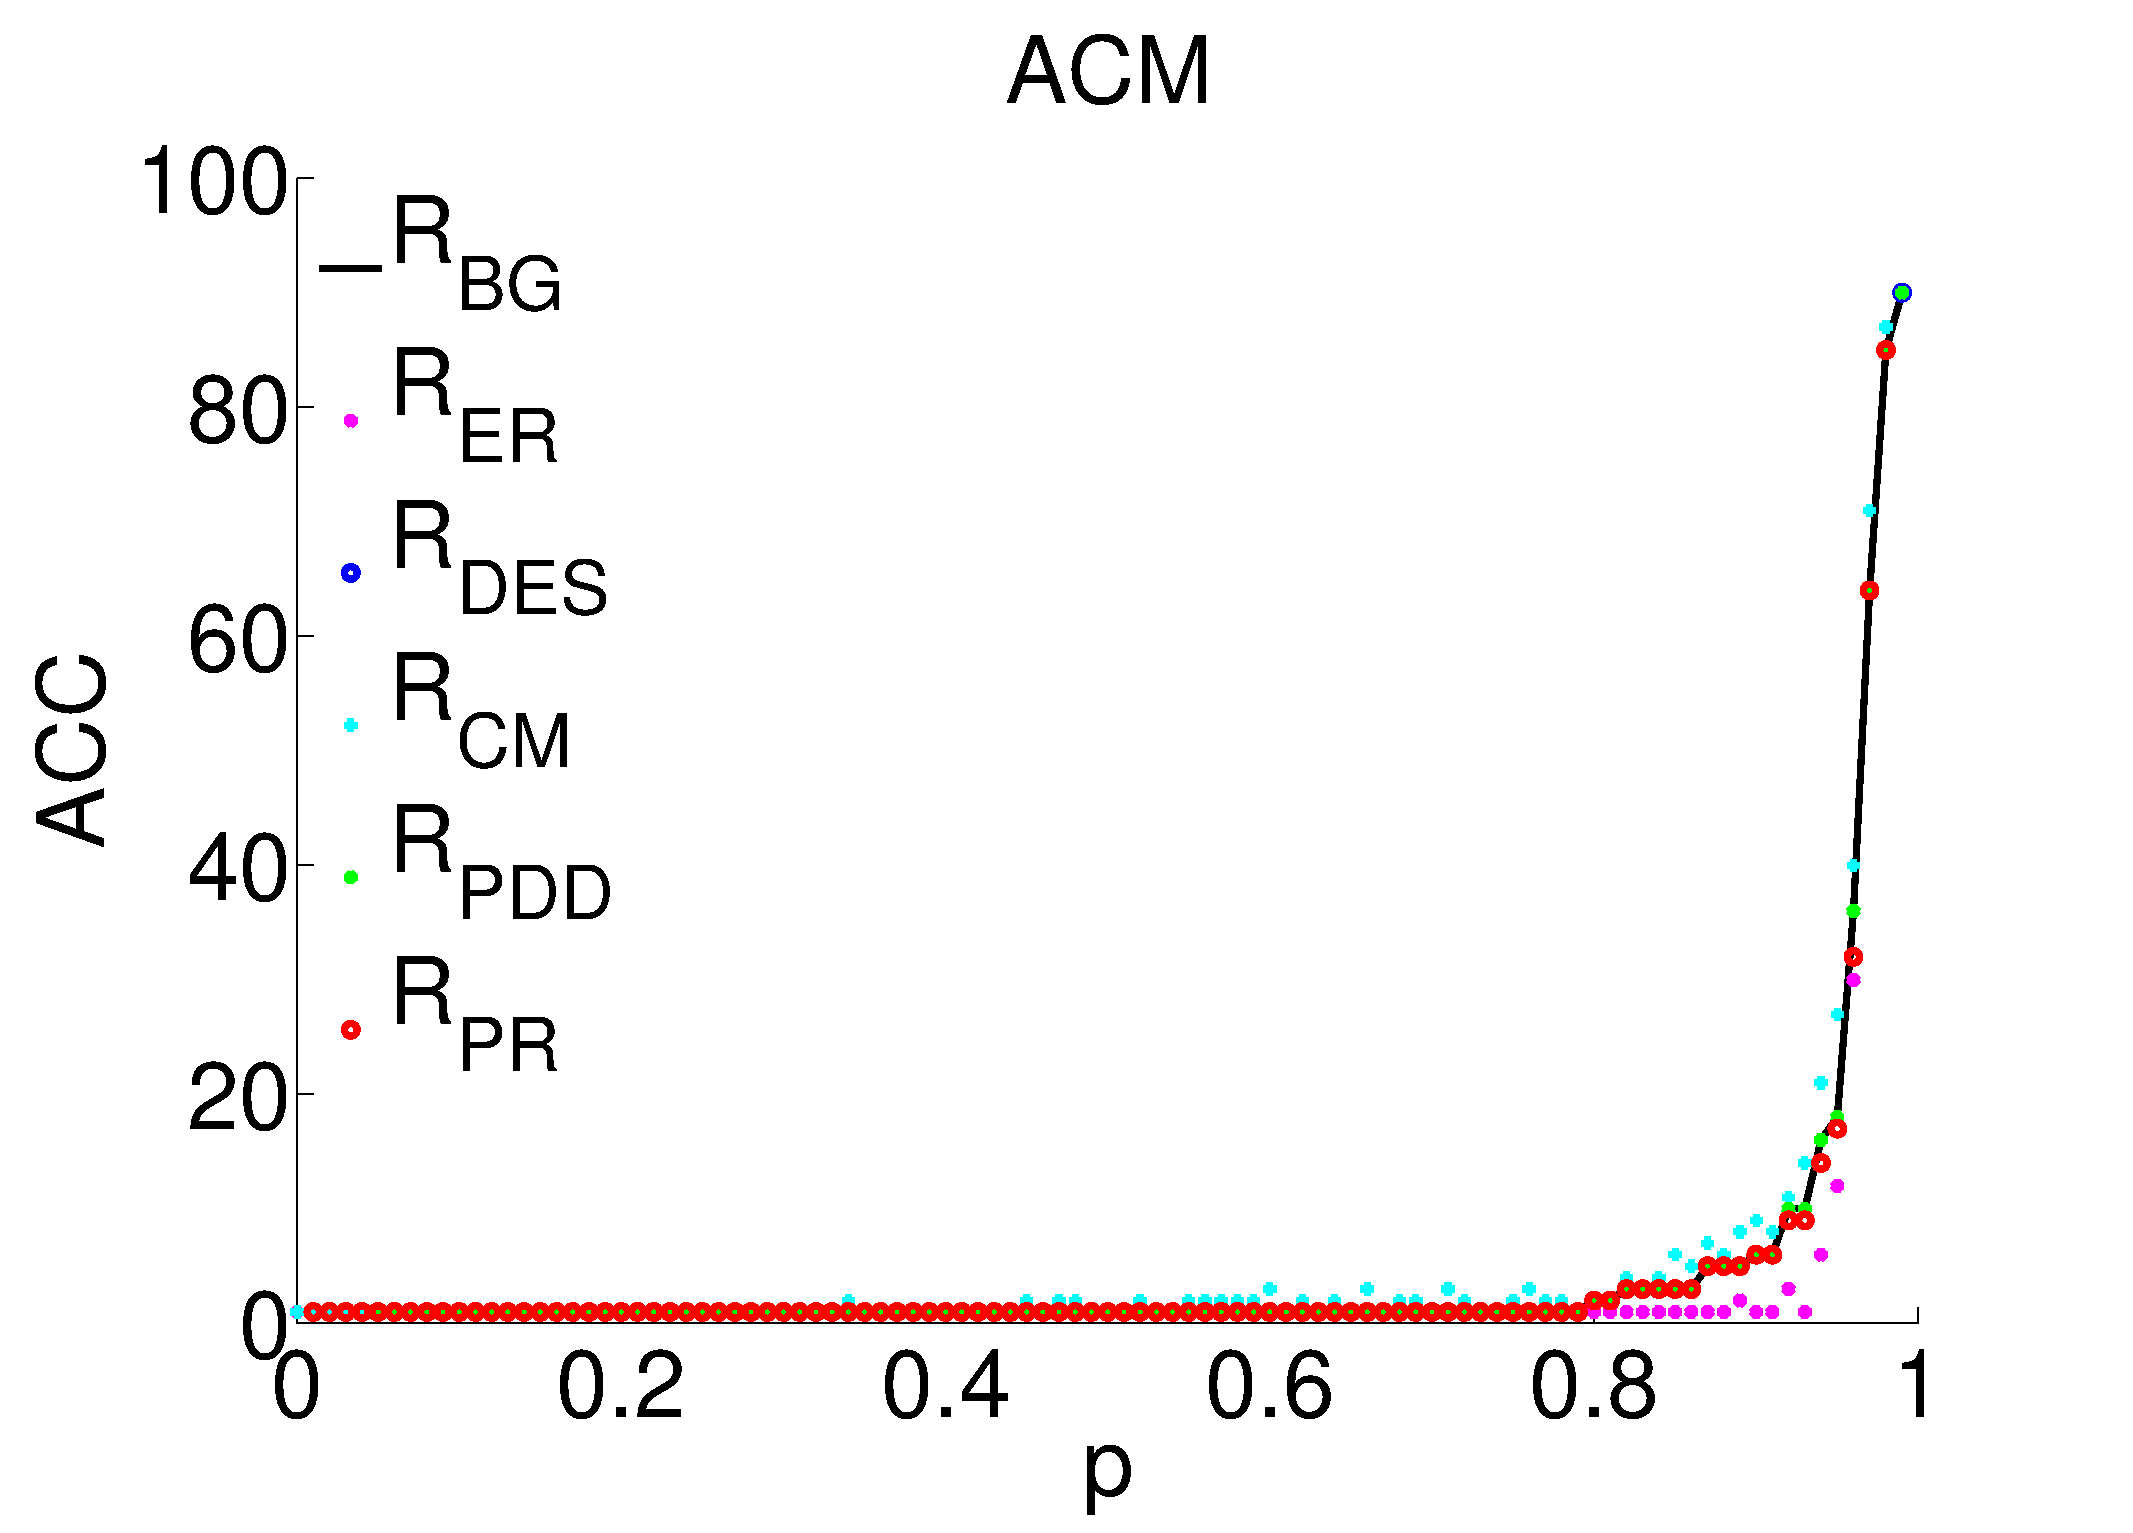
\includegraphics[width=0.49\textwidth]{Figures/connec_compo_ACM.eps}
	\rule{35em}{0.5pt} 
  \caption[Average Connected Components]{Assortativity coefficients of FCM (left) and ACM (right) brain graphs and their random graphs.} 
    \label{fig:Average Connected Components}
 	
\end{figure}

We can expect that the nodes are assumed to be well connected at lower $r$ and $p$, it is always possible to reach any node in the network starting from any other node. That means subgraphs should begin to be constructed after a high $r$ and $p$ values. Average connected components $ACC$ measure is calculated via \textsc{NetworkX} tool for all graphs in this project \citep{XYZNETW}.

Figure B.7 shows that, at higher $r$ and $p$ levels, the nodes become sparse as the network densities get lower in FCM and ACM graphs. When $r>0.95$ and $p=1.00$, we can imagine each node as a single subgraph, since none of the nodes is connected and therefore $ACC$ becomes equals to 90, which is exactly the total number of nodes in all graph types. 


\section{Degree Distribution}
Degree distribution of a network $p(k)$ reflects the probability of a node to have a given number of degree $k$. Figures B.8 and B.9 illustrates $p(k)$ for functional connectivity map (FCM) and anatomical connectivity map (ACM) related brain graphs and their randomized networks. It can be seen that, at lower threshold $r$- or probability $p$-values (here, $p$ is used to generate the adjacency matrix), the networks tend to be highly dense by means of number of edges in graph (see Section 2.4.1 and Figure B.1). For instance, at $r=0$, the probability of any node to have 89 edges $p(k=89)$ is equal to 1.0, each node is connected to all other nodes. At high $r$-values, $p(k=0)$ dominates.    

\begin{figure}[htbp]
 
  \centering
	 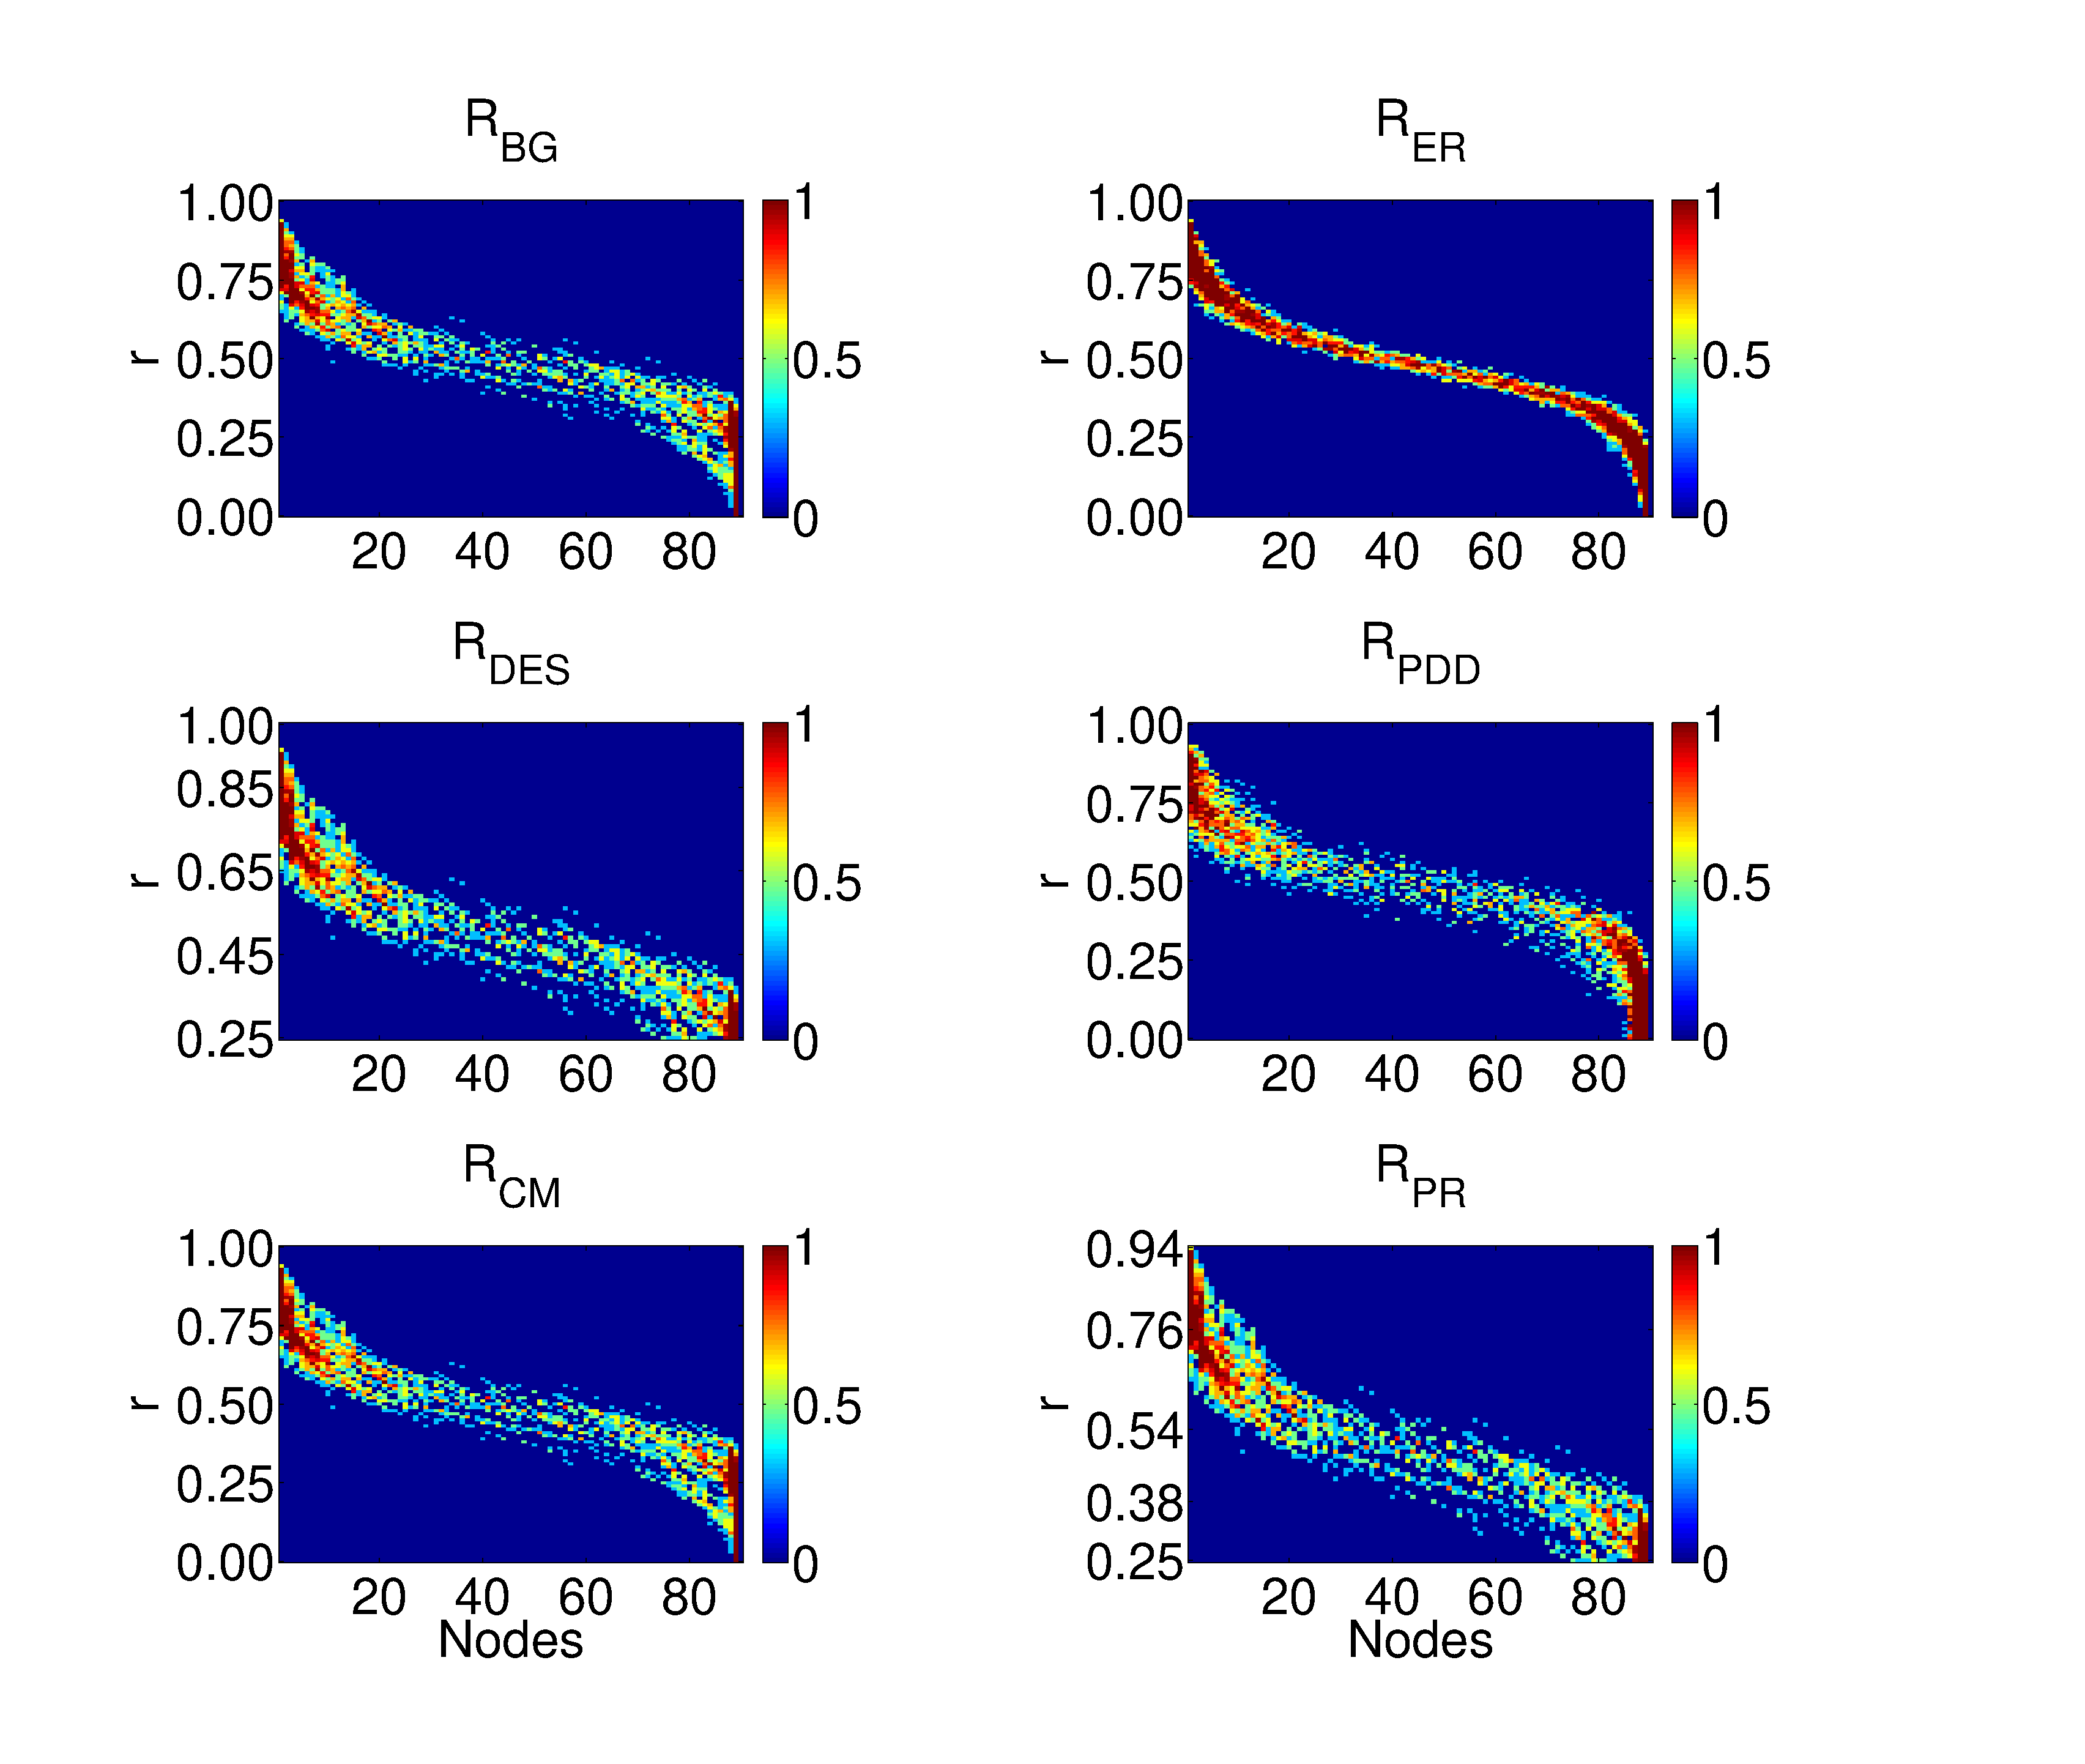
\includegraphics[width=\textwidth]{Figures/Degree_Distribution_Fnc.eps}
	\rule{35em}{0.5pt} 
  \caption[Degree Distribution, FCM]{Heat maps of $p(k)$ of the brain graph $R_{BG}$ constructed on the functional connectivity map obtained from fMRI-BOLD measurement and its randomly generated networks. The limits of colorbar are in logarithmic scale.} 
    \label{fig:Degree Distribution, FCM}
 	
\end{figure}



\begin{figure}[htbp]
 
  \centering
	 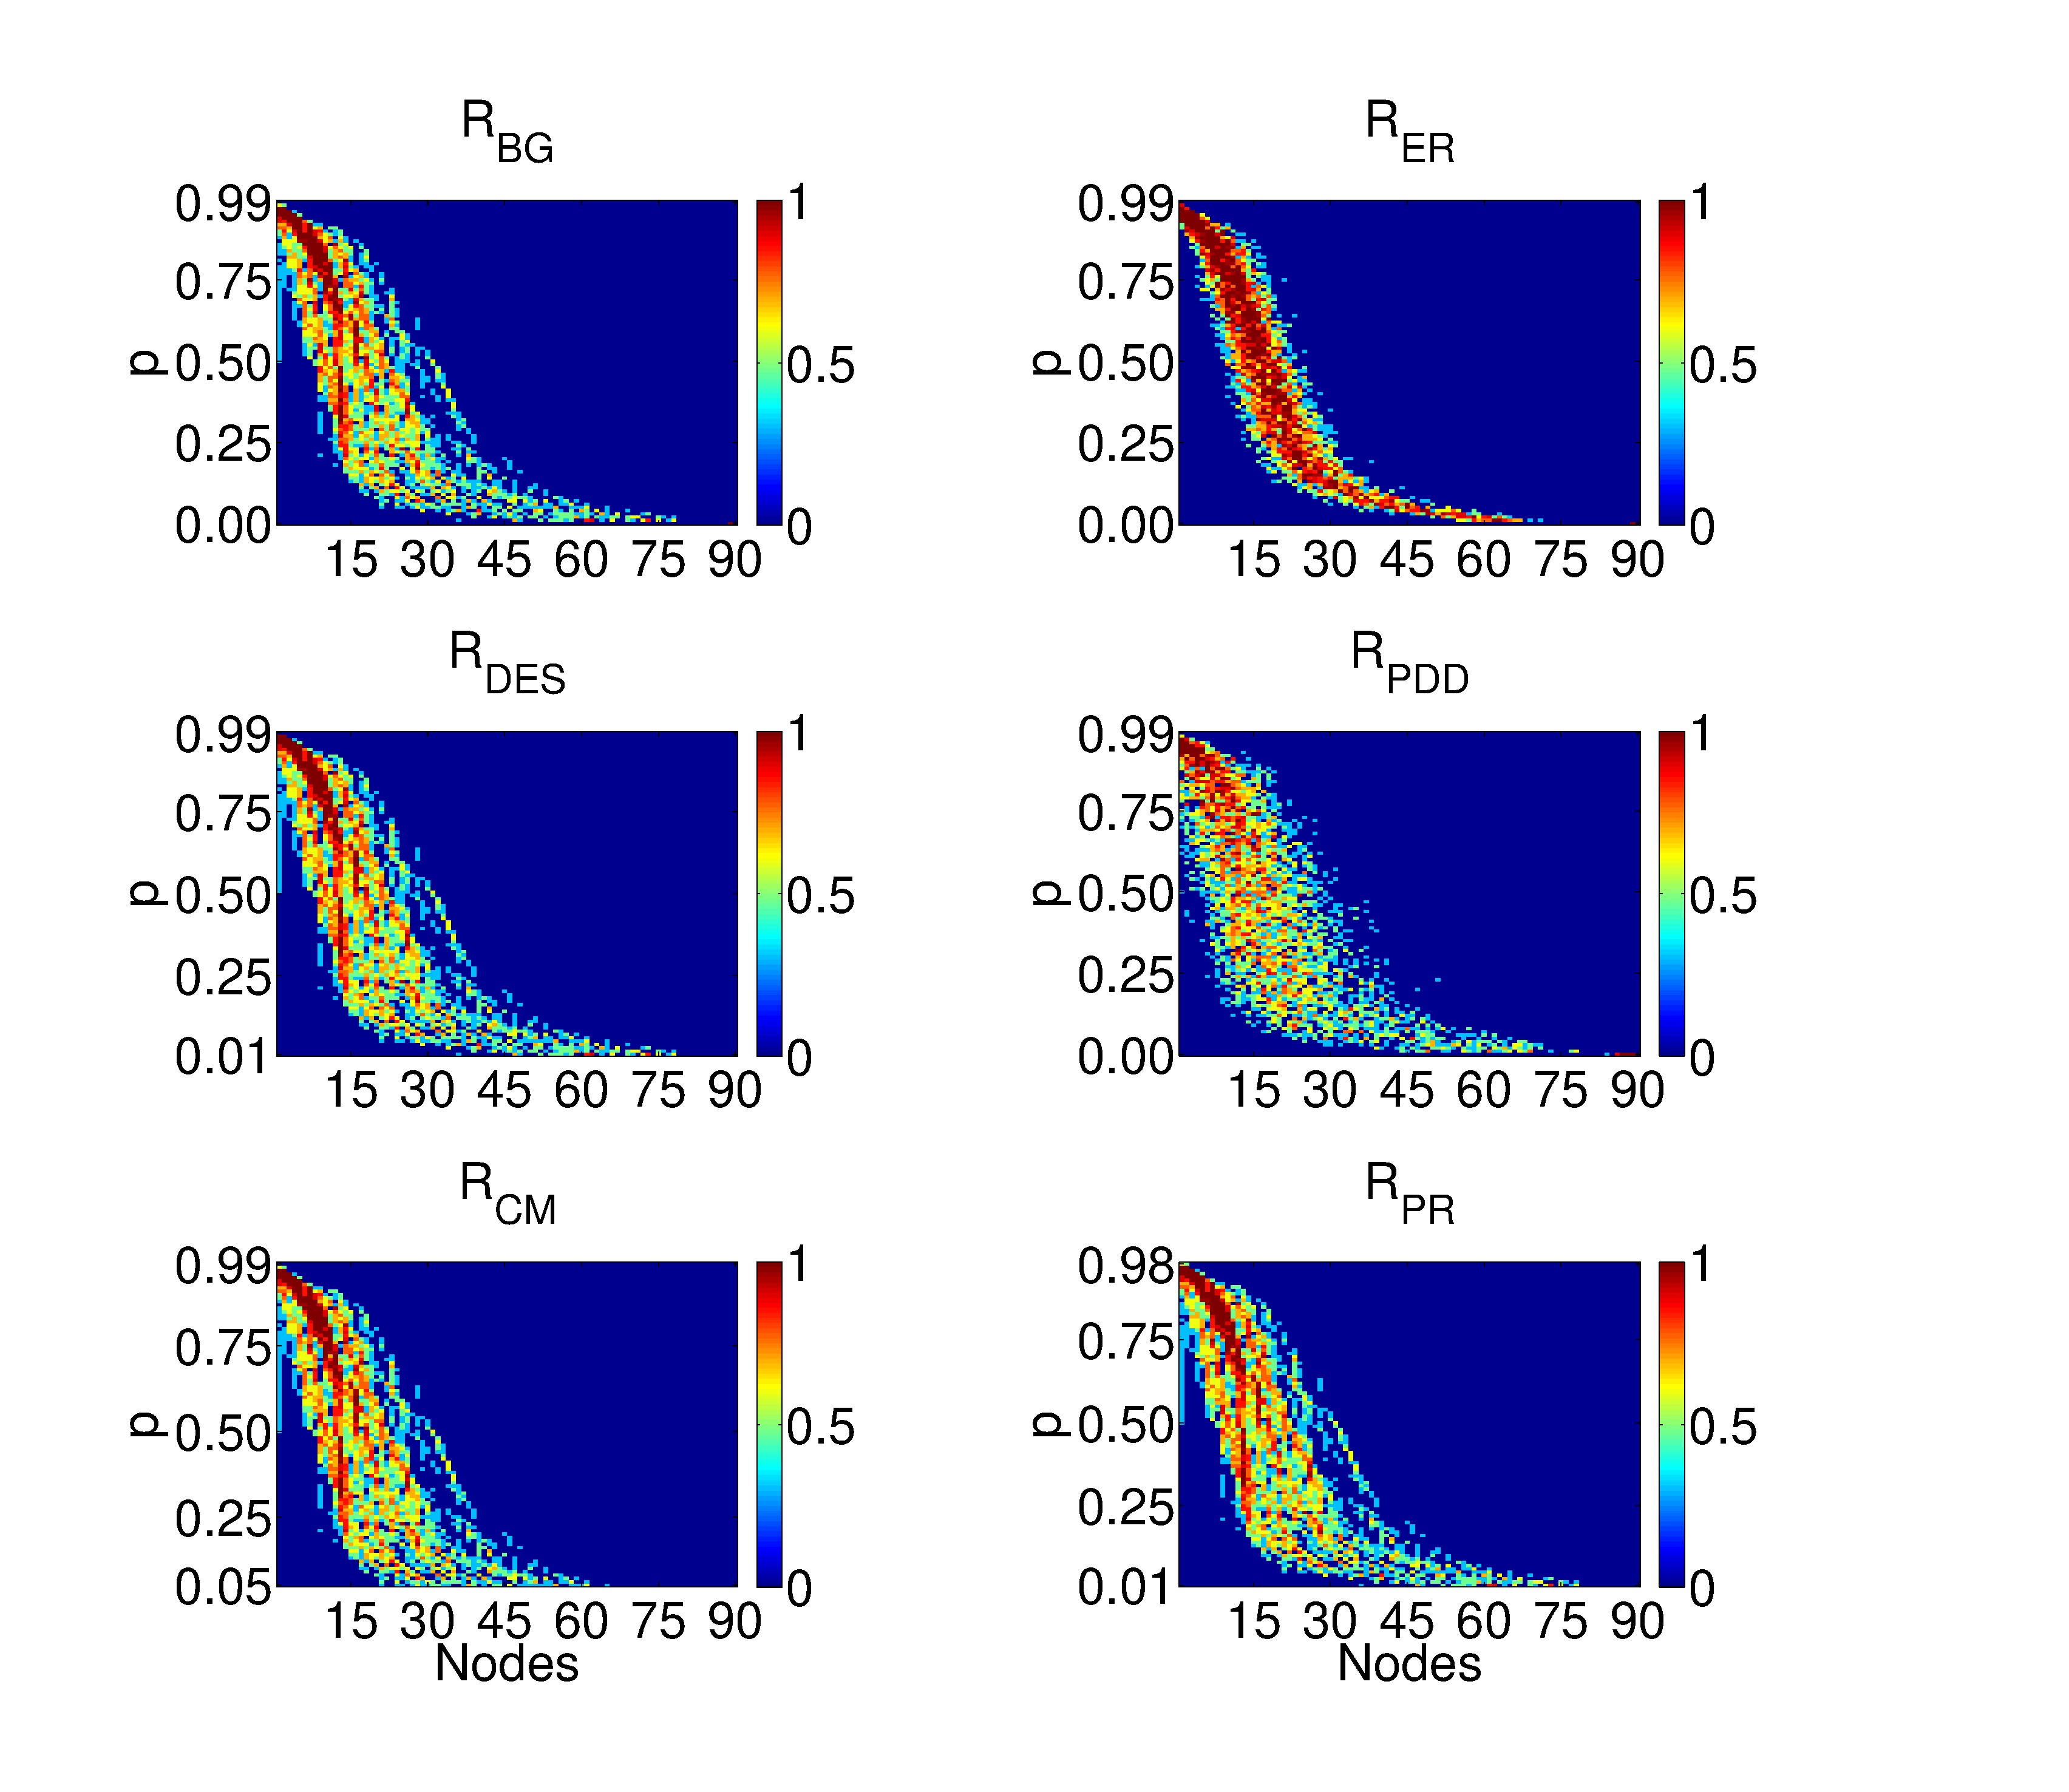
\includegraphics[width=\textwidth]{Figures/Degree_Distribution_Stru.eps}
   \rule{35em}{0.5pt} 
  \caption[Degree Distribution, ACM]{Heat maps of $p(k)$ of the brain graph $R_{BG}$ constructed on the anatomical connectivity map obtained from DW-MRI measurement and its randomly generated networks. The limits of colorbar are in logarithmic scale.} 
    \label{fig:Degree Distribution, ACM}
 	
\end{figure}

\clearpage

\section{Clustering Coefficient of Nodes}

The clustering coefficient of each node $C_i$ is measured as ratio between number of triangles around a node and all possible edge connections of that node $\binom{k_i}{2}$ \citep{WAT98}, 
\begin{equation}
C_i =  \frac{2t_i}{k_i(k_i -1)} \,\, .
\end{equation}
As the number of triangles around a node increased, $C_i$ becomes larger indicating more segregated nodes in the network.
\begin{figure}[htbp]
  \centering
	 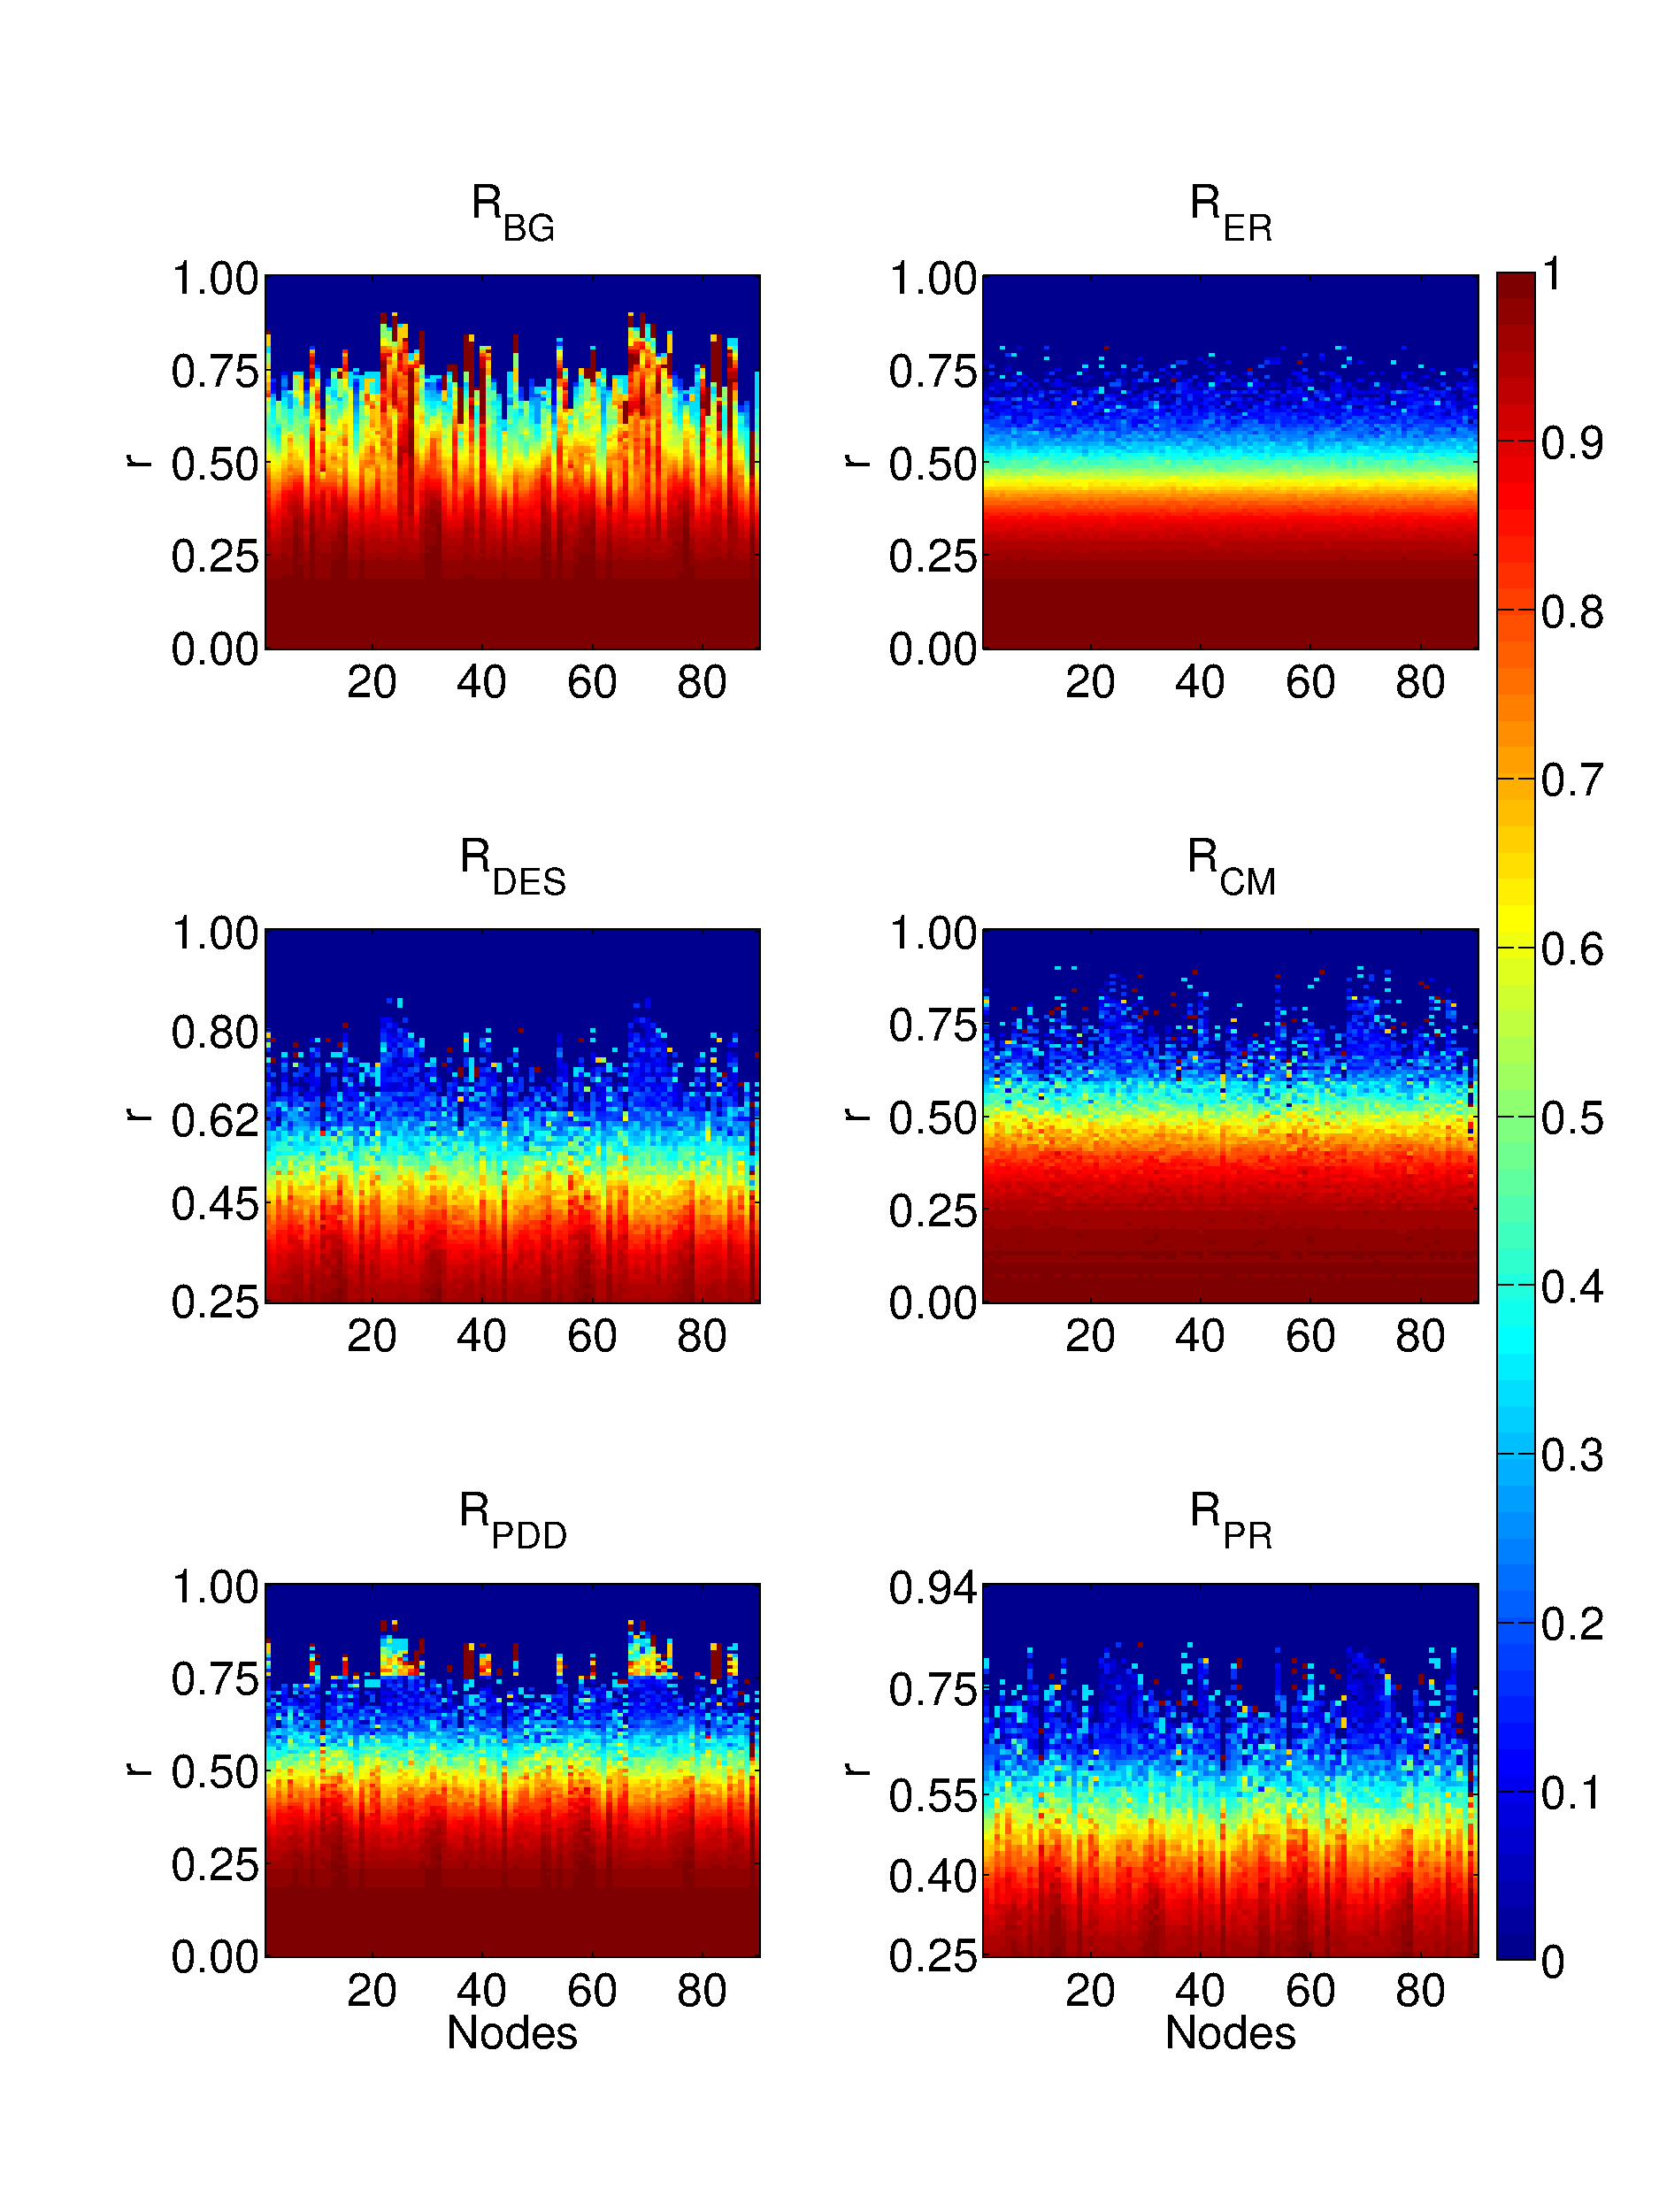
\includegraphics[width=0.9\textwidth, height=155mm]{Figures/Clustering_Coefficient_Nodes_Fnc.eps}
	\rule{35em}{0.5pt}  
  \caption[Clustering Coefficient of Nodes, FCM]{Heat maps of $C_i$ of the brain graph $R_{BG}$, which is constructed on the functional connectivity map obtained from fMRI-BOLD measurement, and its randomly generated networks.} 
    \label{fig:Clustering Coefficient of Nodes, FCM}
 	
\end{figure}

\begin{figure}[htbp]
 
  \centering
	 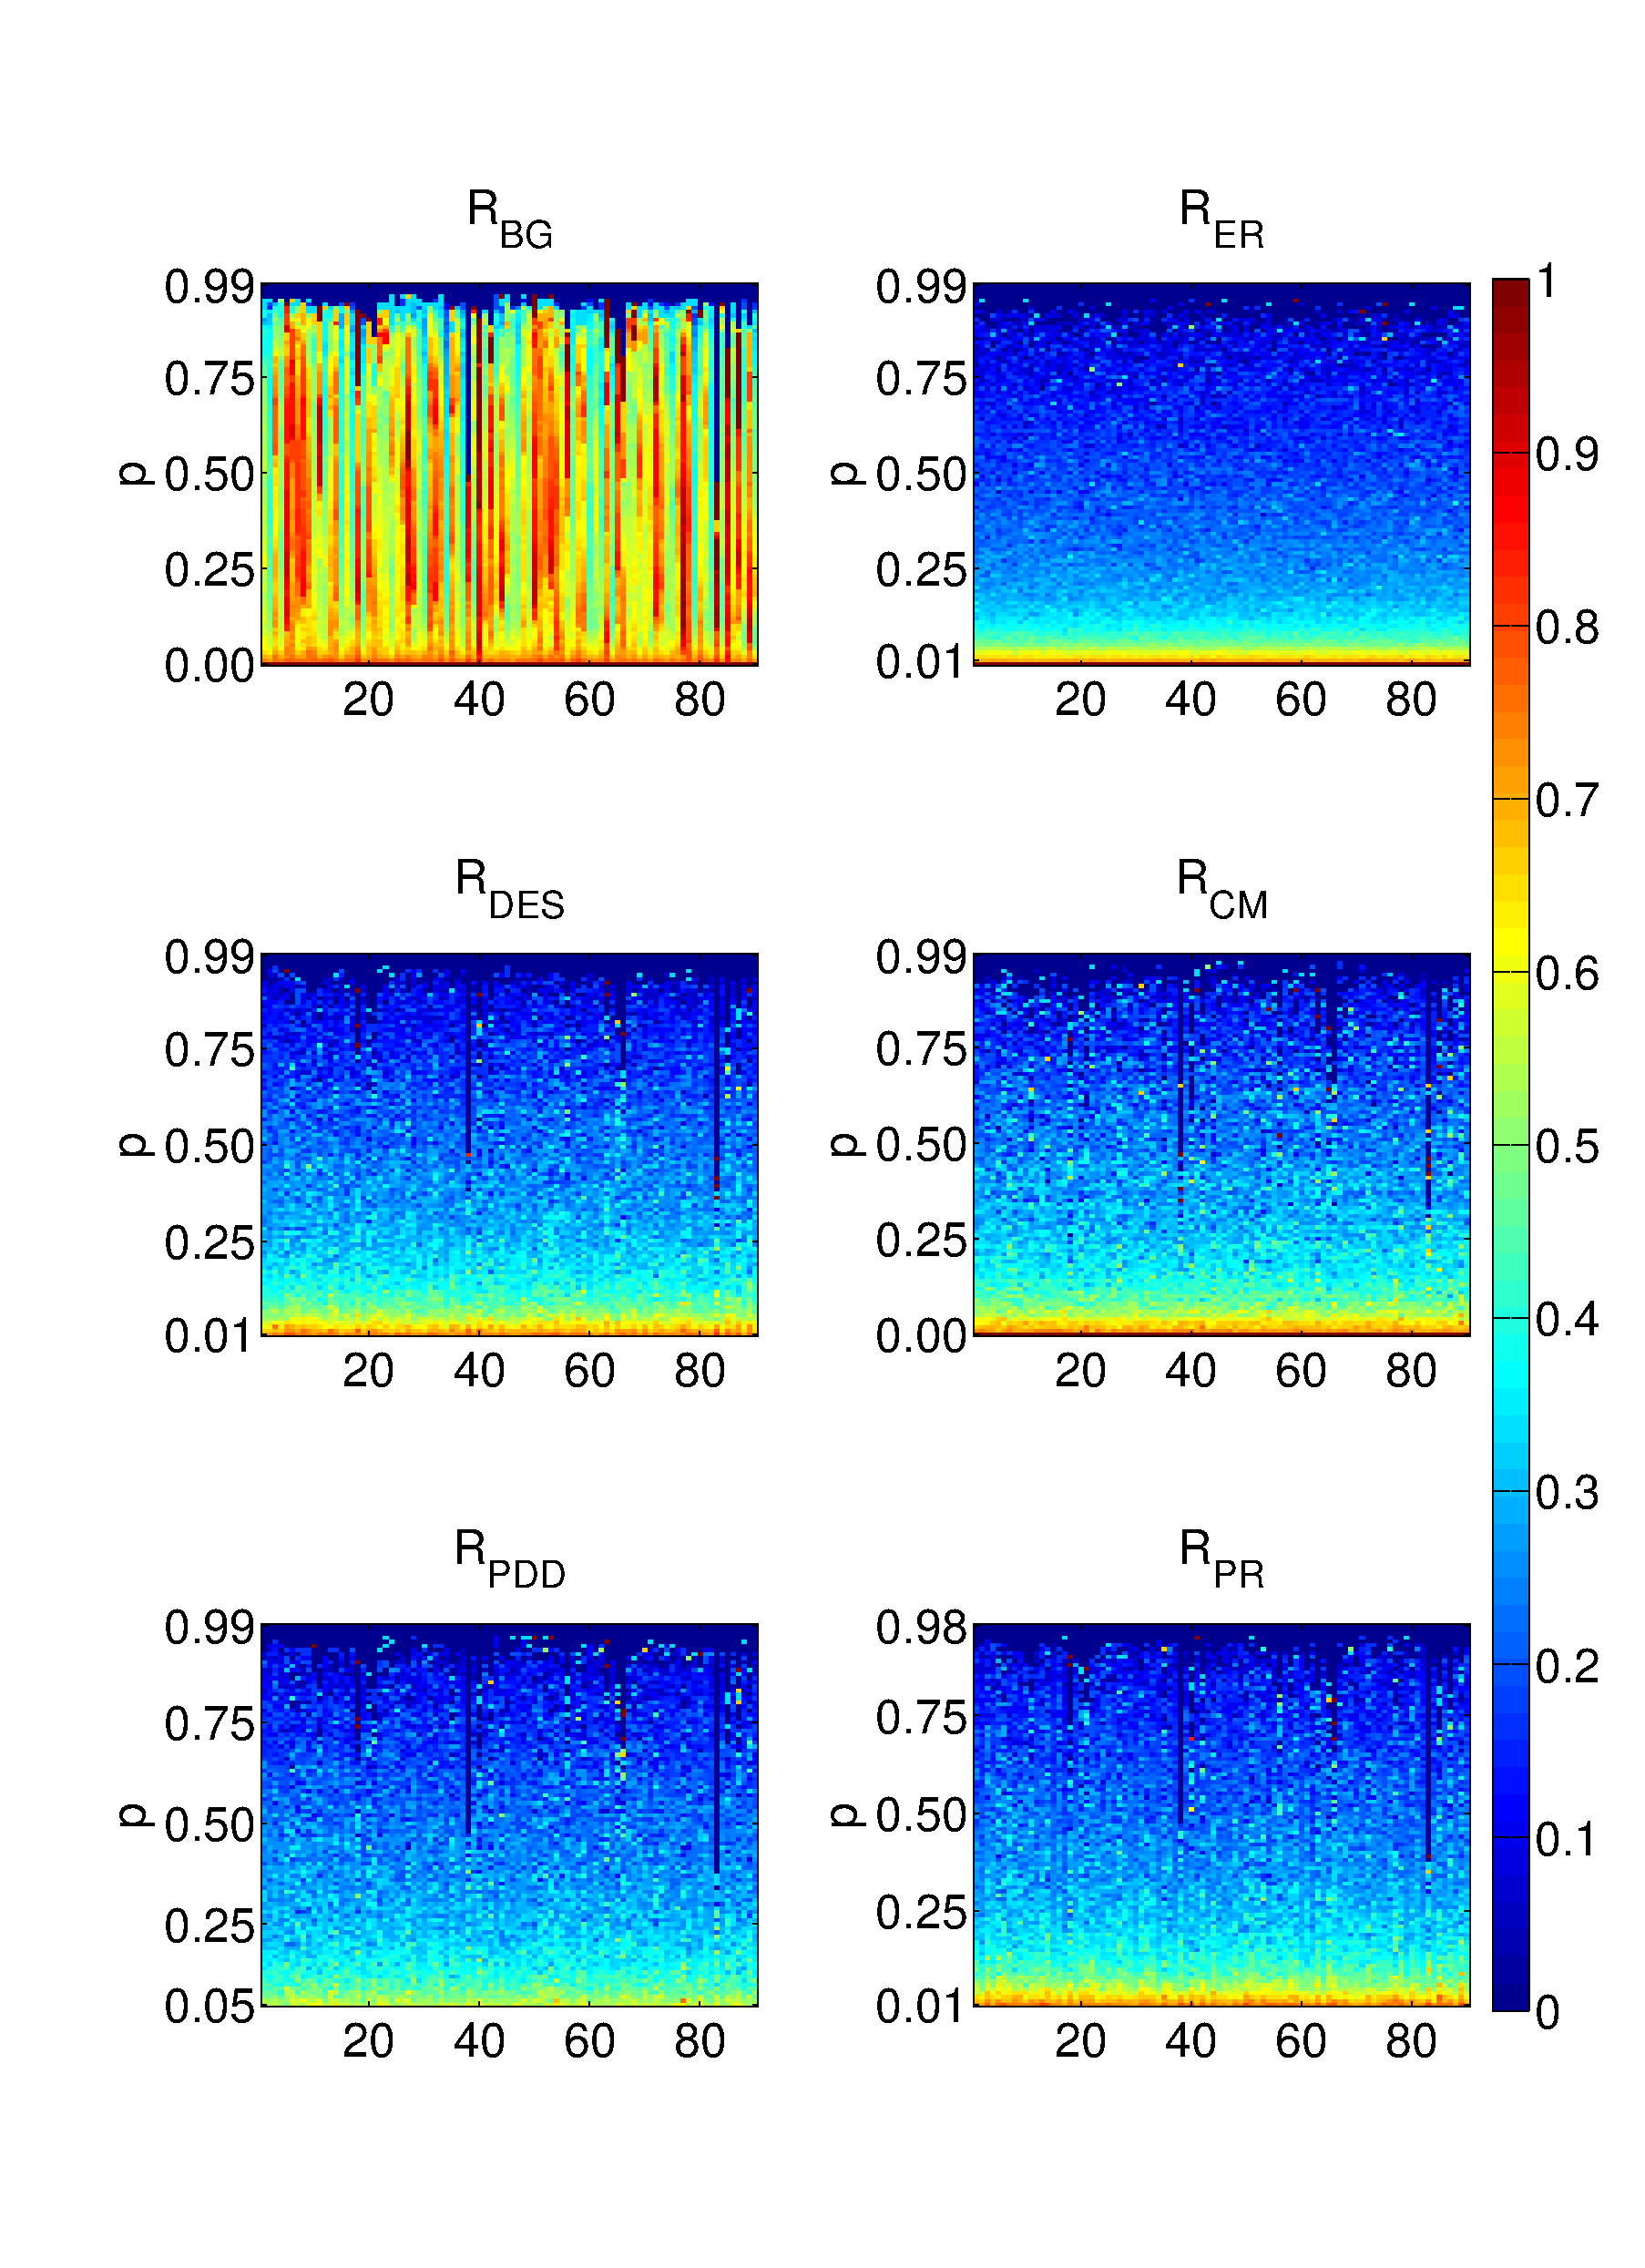
\includegraphics[width=\textwidth]{Figures/Clustering_Coefficient_Nodes_Stru.eps}
	\rule{35em}{0.5pt}  
  \caption[Clustering Coefficient of Nodes, ACM]{Heat maps of $C_i$ of the brain graph $R_{BG}$, which is constructed on the anatomical connectivity map obtained from DW-MRI measurement, and its randomly generated networks.} 
    \label{fig:Clustering Coefficient of Nodes, ACM}
 	
\end{figure}

